
\chapter{Sistemas Fotovoltaicos de Conexión a Red}
\label{cha:SFCR}


\section{Conceptos básicos}

\subsection{Definición de un SFCR}

Un Sistema Fotovoltaico Conectado a la Red (SFCR) es un sistema cuya
función es producir energía eléctrica en condiciones adecuadas para
poder ser inyectada en la red convencional. Como se muestra en la
figura \ref{fig:EsquemaSFCR}, un SFCR se compone del generador
fotovoltaico, un inversor DC/AC y un conjunto de protecciones
eléctricas. 
\nomenclature[SFCR]{SFCR}{Sistema fotovoltaico de
  conexión a red} 

%
\begin{figure}
\includegraphics{../figs/EsquemaSFCR}

\caption{Esquema de un SFCR.\label{fig:EsquemaSFCR}}

\end{figure}

La energía producida por este sistema será consumida parcial o
totalmente en las cercanías, y la energía sobrante será inyectada en
la red para su distribución a otros puntos de consumo. Es común que
existan mecanismos de retribución económica que compensan al
propietario del sistema por la energía que su sistema intercambia con
la red. Pueden distinguirse, de forma simplificada, dos esquemas: la
retribución con prima (\emph{feed-in tariff}) y el balance neto
(\emph{net-metering}). 

En el mecanismo de retribución con prima\footnote{Este
mecanismo es de uso común en los países europeos. La referencia
\cite{Collado2009} proporciona información sobre el uso de este
mecanismo en diferentes países europeos, donde es frecuentemente
implementado.}, generalmente el propietario
del SFCR recibe ingresos derivados de la energía total producida
(independientemente de la que haya sido consumida en las cercanías del
SFCR). En este caso, el diseño no necesita considerar un consumo a
satisfacer, como sí será el caso en los sistemas autónomos o de
bombeo. Con este mecanismo, el objetivo del diseñador es que la
producción anual del sistema sea la máxima posible sin tomar en
consideración los consumos cercanos (siendo posible instalar un SFCR
sin ningún consumo asociado). Este mecanismo favorece la implantación
de los sistemas fotovoltaicos cuando el coste de la energía producida
es superior al de la tarifa eléctrica convencional (sin tener en
consideración las externalidades ambientales). Aunque formalmente
favorece la generación distribuida, sin ningún condicionante adicional
puede ocasionar un crecimiento desordenado que disocie las ubicaciones
de los sistemas fotovoltaicos de los centros de consumo. 

El mecanismo de balance neto\footnote{Este mecanismo es la elección
habitual en los Estados Unidos de América. La referencia \cite{Chapman.Rose2011}
detalla las diferentes modalidades empleadas en varios estados.} compensa los saldos de energía eléctrica
entre el SFCR y un sistema de consumo asociado. Cuando la producción
del SFCR supera al consumo, la red eléctrica\footnote{En este
  mecanismo la red eléctrica puede ser asimilada a un sistema de
  almacenamiento infinito. Cabe la posibilidad de repercutir los
  costes asociados a este almacenamiento al propietario del SFCR
  mediante peajes o algún esquema similar.} absorbe el excedente
puntual, generándose derechos de consumo diferido para el propietario
del SFCR. Estos derechos de consumo se pueden ejercer cuando la
producción del SFCR no es suficiente para satisfacer el consumo
asociado. La interacción entre el SFCR, el consumo y la red bajo este
mecanismo de retribución favorece la generación distribuida y la
gestión de la demanda\footnote{Más información en el vídeo de las
  jornadas ``Competitividad de las energías renovables. Autoconsumo y
  Balance Neto'' \url{http://www.eoi.es/mediateca/video/1331} y en los
  documentos de la Jornada ``El Autoconsumo Fotovoltaico en España''
  \url{http://asif.org/2011/09/jornada-solar-fotovoltaica-el-autoconsumo-fotovoltaico-en-espana/}.}.
El diseño de un SFCR en el contexto de este mecanismo debe incluir el
consumo asociado como una variable adicional que condicionará el
tamaño del generador fotovoltaico. 

Salvo afirmación expresa en contra, a lo largo de este capítulo se
supondrá que el SFCR se enmarca en un mecanismo de retribución con
prima y, por tanto, se obviará el consumo asociado.

\subsection{Características distintivas de SFCR sobre suelo y en edificación}

Tradicionalmente se distingue entre SFCRs instalados sobre suelo y
en edificación. Dentro de los instalados sobre suelo existen los sistemas
estáticos, con una inclinación y orientación fija, y los sistemas
de seguimiento, que varían la posición del generador a lo largo del
día y año para maximizar la radiación efectiva incidente. En los instalados
sobre edificación es frecuente diferenciar los sistemas según el grado
de integración del sistema con el edificio. Así, el documento HE5
del Código Técnico de la Edificación considera tres casos en lo que
a disposición de módulos se refiere: general, superposición de módulos
e integración arquitectónica. Considera que existe integración arquitectónica
cuando los módulos cumplen una doble función energética y arquitectónica
y además sustituyen elementos constructivos convencionales o son elementos
constituyentes de la composición arquitectónica. Se supone que existe
superposición arquitectónica cuando la colocación de los módulos se
realiza paralela a la envolvente del edificio.


\subsubsection{SFCR sobre suelo}

El diseño de un SFCR sobre suelo tiene como objetivo maximizar la
producción energética anual del sistema con el menor coste y la menor
ocupación de terreno posibles. Como primera clasificación distinguiremos
entre los sistemas estáticos, aquellos cuya inclinación y orientación
permanece inalterable, y los sistemas de seguimiento.

El fundamento de los sistemas de seguimiento es doble: en primer lugar,
la radiación incidente aumenta al seguir al sol; además, las pérdidas
por reflexión disminuyen si el apuntamiento al sol mejora. Por tanto,
el objetivo de estos sistemas es reducir el ángulo formado entre la
línea que une el generador con el sol y la perpendicular al plano
del módulo y así apuntar al sol a lo largo de su movimiento celeste.
Las diferentes técnicas de seguimiento buscan concretar ese objetivo
general sacrificando un apuntamiento perfecto en aras de conseguir
sistemas estructurales más económicos y mejores aprovechamientos del
terreno. 

Así, el mejor método de seguimiento desde la perspectiva de la producción
eléctrica es el denominado a doble eje, que consigue apuntar al sol
con precisión a lo largo de todo su recorrido. En el siguiente puesto
de los que optimizan la producción destaca el seguimiento acimutal,
que sacrifica un movimiento (inclinación del generador) para conseguir
sistemas más económicos. El método consiste en girar de este a oeste
sobre un eje vertical. Su uso está decreciendo en comparación al método
de doble eje. Otro planteamiento diferente es el utilizado por el
seguimiento polar. El único eje sobre el que se produce el giro está
inclinado de forma paralela al eje de rotación de la Tierra, consiguiendo
que el generador aparezca al sol como perpendicular a sus rayos durante
gran parte del recorrido. No obstante, las complicaciones estructurales
y de giro, y la dificultad de su implantación en grandes plantas han
provocado que su uso sea ocasional. Por último se debe mencionar el
método de seguimiento horizontal con eje Norte-Sur. Sus ventajas son
la sencillez y estabilidad estructural (el eje es horizontal y paralelo
al terreno, con tantos puntos de apoyo como se consideren necesarios),
la facilidad de motorización, así como el mejor aprovechamiento del
terreno en relación a un sistema de doble eje.

El lector interesado en sistemas de seguimiento podrá encontrar mayor
información al respecto y un conjunto de ecuaciones que describen
los diferentes métodos en \cite{Perpinan2008}. 

El mejor aprovechamiento de terreno depende directamente del porcentaje
de radiación que quedará sombreada por los seguidores cercanos, lo
que se conoce como sombras mutuas. En general, cuanto más exacto es
el método de seguimiento, menos eficiente es su aprovechamiento de
terreno: para un mismo valor de radiación sombreada, la separación
entre seguidores aumenta en sistemas que apuntan mejor. De ahí que
los sistemas estáticos sean la opción preferida cuando el terreno
disponible sea limitado y se desee alcanzar una potencia instalada
determinada (por ejemplo para aprovechar toda la capacidad que ofrece
el punto de conexión concedido) o limitar la inversión económica a
costa de reducir la productividad del sistema.

Recordando que en un SFCR sobre suelo el objetivo es obtener el menor
coste de la energía producida durante su vida útil con la menor ocupación
de terreno posible, el diseñador debe configurar el generador (principalmente
su tamaño y tipo de seguimiento) teniendo en cuenta al menos tres
factores:
\begin{itemize}
\item La inversión económica que es posible realizar, relacionada principalmente
con la potencia del generador%
\footnote{También deberá tener en cuenta la limitación de potencia que impone
las características del punto de conexión concedido por la compañía
eléctrica.} y con el tipo de seguimiento empleado.
\item El rendimiento económico deseado, relacionado con la energía producida
por el sistema y, por tanto, con el modo de seguimiento empleado y
con la radiación disponible. 
\item La ocupación de terreno, relacionado con el modo de seguimiento empleado.
\end{itemize}
Es ciertamente dificil establecer recomendaciones de aplicación
universal. En \cite{Perpinan2012} se propone un método para optimizar
la separación entre seguidores teniendo en cuenta las consideraciones
previas.

Los sistemas de seguimiento han proliferado en España en los últimos
años. Sin embargo, debido a un contexto reciente de bajos precios de
módulos, ya no son la opción más frecuente: la mayor productividad
ofrecida ya no supera tan ampliamente sus contraprestaciones de mayor
ocupación de terreno y, principalmente, mayor inversión.

Los sistemas instalados sobre suelo frecuentemente superan la potencia
de $\SI{100}{\kilo\watt}$, y en varios casos superan los $\SI{50}{\mega\watt}$,
y por tanto, suelen contar con una instalación de evacuación en Media
Tensión. En este tipo de SFCR una proporción importante del trabajo
de ingeniería se dedica al diseño del sistema de interconexión de los
módulos para formar el generador, el sistema eléctrico que conecta
el generador con los equipos inversores, el sistema de evacuación
a red de la energía producida y la red de tierras.


\subsubsection{SFCR en edificación}

El diseño de un SFCR en edificación es frecuentemente más complejo
que el de un SFCR sobre suelo. La integración del sistema fotovoltaico
con el edificio exige tener en cuenta muchos factores que condicionan
la ubicación y la configuración del generador. Así, la orientación
e inclinación del generador ya no puede ser elegida para optimizar
la producción energética sino que las características propias del
edificio y de los elementos que alberga obligan muy frecuentemente
a optar por ángulos que difieren del óptimo. En este tipo de sistemas,
el diseñador debe tomar las decisiones oportunas para aprovechar las
sinergias entre edificio y sistema fotovoltaico, reduciendo las posibles
interferencias entre uno y otro. Por ejemplo, un generador fotovoltaico
puede ser instalado como toldo fijo sobre ventanas reduciendo la insolación
que entra en el edificio y por tanto, disminuyendo la carga térmica
en el mismo. La ubicación del generador vendrá determinada por la
orientación de la fachada que se pretende sombrear, su inclinación
será un compromiso entre la producción energética del SFCR y la cantidad
de sombra deseada, y el tamaño del generador dependerá del área acristalada
a sombrear. 
% Es recomendable acudir a la referencia \cite{PV-database}
% para contemplar las variadas posibilidades de uso de sistemas fotovoltaicos
% en edificios.

Para las instalaciones fotovoltaicas en edificación es de particular
importancia el documento HE5 del Código Técnico de la
Edificación \cite{CTE2017}.
Esta normativa obliga a incorporar sistemas fotovoltaicos cuando se
superan los $\SI{5000}{\meter\squared}$ construidos. La potencia
nominal de estos sistemas (potencia de inversor) queda determinada por
la ecuación \ref{eq:PotenciaCodEdificacion}:

\begin{equation}
P_{min}=C\cdot(0.002\cdot S - 5)
\label{eq:PotenciaCodEdificacion}
\end{equation}
siendo $P_{min}$ la potencia nominal\footnote{Definida como la ``suma
  de la potencia nominal de los inversores (la especificada por el
  fabricante) que intervienen en las tres fases de la instalación en
  condiciones nominales de funcionamiento.''} a instalar
($\si{\kilo\W}$), $S$ la superficie construida en metros cuadrados y
$C$ un coeficiente relacionado con la zona climática en la que se
ubica el edificio.  En todo caso, la potencia nominal máxima
obligatoria será de $\SI{100}{\kilo\watt}$.

Este documento divide España en cinco zonas climáticas de acuerdo al
valor medio anual de la radiación global diaria en el plano
horizontal.  Por ejemplo, toda la cornisa cantábrica está encuadrada
en la zona I (radiación inferior a $\SI{3.8}{\kWh\per\meter\squared}$)
mientras que Canarias y parte de Andalucía pertenecen a la zona V
(radiación superior a $\SI{5}{\kWh\per\meter\squared}$) . El
coeficiente $C$ de la ecuación \ref{eq:PotenciaCodEdificacion} toma un
valor de 1 para la zona I y un valor de 1.4 para la zona V, de forma
que este Código aboga por instalar mayor potencia en las zonas con
mayor radiación.

En los apartados \ref{sub:Orientacion-e-inclinacion} y
\ref{sub:Sombras-lejanas} se discute sobre los requisitos que
este documento exige para la disposición de módulos y sombras en el
generador.

Los sistemas instalados en edificación no suelen superar la potencia
de $\SI{100}{\kilo\watt}$. Su interconexión con la red eléctrica se
realiza frecuentemente en Baja Tensión, aunque esta opción no siempre
es posible, ya sea por superar el límite de potencia o por
imposibilidad de acceso a un punto de conexión de BT cercano.

Las condiciones técnicas de conexión a la red eléctrica de los
sistemas de autoconsumo en España se detallan en la ``Guía Técnica de
Aplicación del REBT: Instalaciones Generadoras de Baja Tensión
(ITC-BT-40)''\footnote{Accesible en
  \url{https://industria.gob.es/Calidad-Industrial/seguridadindustrial/instalacionesindustriales/baja-tension/Paginas/guia-tecnica-aplicacion.aspx}.},
y en el anexo III (Modos de Conexión) de la ``Guía Profesional del
Autoconsumo''\footnote{Disponible en
  \url{https://www.idae.es/publicaciones/guia-profesional-de-tramitacion-del-autoconsumo}.}
publicado por el IDAE. En estos documentos se recopila el catálogo de
posibilidades de conexión y modos de medición según el tipo de
autoconsumo (individual o colectivo) y tipo de conexión (en red
interior o a través de red).


En este tipo de SFCR el diseño de los sistemas eléctricos debe tener
en cuenta las canalizaciones previstas o existentes en el edificio.
Por facilidad de instalación y mantenimiento, y por seguridad de los
sistemas, es recomendable el uso de canalizaciones separadas del resto
de sistemas del edificio. Sin embargo, los criterios de seguridad
eléctrica aconsejan utilizar una red de tierras común para el edificio
y el sistema fotovoltaico. Una proporción importante del trabajo de
ingeniería se dedica a ubicar correctamente el generador para
maximizar la producción y minimizar el efecto del sombreado, y a
diseñar y elegir los elementos de anclaje de los módulos al edificio.


\subsubsection{Sistemas de concentración}

En los sistemas de concentración%
\footnote{Un sistema de concentración es aquel que, para obtener reducción de
costes, reduce el tamaño del material activo (en este caso, la célula
fotovoltaica) y emplean lentes que concentran la radiación solar.
De esta forma, la potencia eléctrica por área expuesta es teóricamente
similar (despreciando las pérdidas debidas a la lente y al acoplamiento)
a la de un módulo convencional empleando menos material semiconductor.%
} es imprescindible adoptar el seguimiento a doble eje, ya que los
concentradores, grosso modo, son ciegos a la radiación difusa y tan
sólo son capaces de aprovechar la componente directa de la radiación.
La concentración de radiación, una tecnología madura ampliamente empleada
en los sistemas de energía solar de alta temperatura, tiene aún una
importancia discreta dentro de los SFCR. La razón de su utilización,
esto es, reducir costes empleando menos material activo, es todavía
un objetivo por alcanzar. Cabe destacar que el material semiconductor
requerido en estos módulos es actualmente más caro que el silicio
empleado en los módulos convencionales. Además, los sistemas fotovoltaicos
de concentración, y particularmente los que optan por altos índices
de concentración (500x a 1000x) son más sensibles al desapuntamiento,
sombras mutuas y suciedad que los sistemas convencionales. Por otra
parte, debe tenerse en cuenta que sólo pueden emplearse allí donde
la proporción anual de radiación directa sea muy elevada. En los últimos
años se han llevado a cabo diferentes iniciativas para aumentar el
número de instalaciones con sistemas de concentración, particularmente
en España. Por tanto, es necesario estar atentos a la evolución de
esta aplicación.




\section{Inversor DC/AC}
\label{InversorSFCR}

\subsection{Conceptos Generales}

La señal de potencia suministrada por un generador fotovoltaico iluminado
es en tensión continua, que debe ser acondicionada para permitir el
correcto acoplamiento a la red eléctrica. El equipo de acondicionamiento
de potencia, denominado inversor DC/AC%
\footnote{DC son las siglas inglesas de \emph{direct current}, corriente continua,
y AC las correspondientes a \emph{alternating current}, corriente
alterna.%
}, realiza la conversión de continua a alterna cumpliendo con determinados
requisitos de tensión eficaz, frecuencia, distorsión armónica de las
ondas de tensión y corriente, eficiencia y rendimiento, seguridad
eléctrica, etc. 

Como será explicado en un apartado posterior, el inversor generalmente
funciona como fuente de corriente autoconmutada y sincronizada con
la red.


\subsection{Características de un inversor comercial}

La información que se puede obtener de la ficha técnica proporcionada
por el fabricante de un inversor puede incluir los siguientes parámetros:
\begin{itemize}
\item Potencia nominal y máxima, siendo ésta un porcentaje de sobrecarga
que el equipo es capaz de soportar durante un determinado período
de tiempo (indicado por el fabricante).
\item Ventana de búsqueda del Punto de Máxima Potencia (MPP en siglas inglesas):
es el rango de tensiones en las que el inversor aplica un algoritmo
de búsqueda del MPP del generador fotovoltaico. Cuando este punto
permanece fuera de esta ventana, el inversor fija en el generador
FV la tensión correspondiente al valor límite de la ventana. Por tanto,
configurar un generador de forma que el MPP recaiga fuera de esta
ventana con cierta frecuencia no tiene consecuencias perniciosas para
el inversor, pero ocasiona pérdidas energéticas variables según la
frecuencia de este hecho.
\item Tensión máxima de entrada: es la máxima tensión que el inversor puede
aguantar sin sufrir una avería. A diferencia de la ventana de tensiones
anterior, sobrepasar esta tensión tiene consecuencias importantes
sobre algunos componentes de entrada del inversor. 
\item Tensión nominal de salida: es la tensión de red a la que se puede
conectar el inversor (habitualmente $\SI{230}{V_{dc}}$ para equipos
monofásicos y $\SI{400}{V_{ac}}$ para equipos trifásicos).
\item Eficiencia máxima: máximo valor que toma la relación entre potencia
de salida y potencia de entrada. En inversores de calidad la eficiencia
es estable en un amplio rango de funcionamiento del equipo y de un
valor cercano a la eficiencia máxima.
\item Rendimiento europeo: es la relación entre la energía entregada por
un inversor que recibe una energía producida por un generador fotovoltaico
funcionando en unas condiciones de radiación características de la
zona centroeuropea. Este parámetro fue propuesto con el objetivo de
poder comparar equipos de diferentes fabricantes con un criterio de
calidad energética. Debe tenerse en cuenta que su valor está ligado
a unas condiciones de radiación determinadas y, por tanto, no puede
aplicarse sin corrección previa al cálculo de producción en lugares
con diferente insolación.
\item Umbral de arranque: según las unidades en las que se expresa, puede
indicar la radiación solar incidente en el generador (W/m\texttwosuperior{})
o la potencia de entrada (W) necesaria para que el inversor comience
el proceso de conversión.
\end{itemize}

\subsection{Tipos de inversores}

A grandes rasgos, los inversores pueden agruparse en tres categorías:
\begin{itemize}
\item Inversor central: un único inversor dedicado a todo el generador (o
a un conjunto de ramas)
\item Inversor orientado a rama (\emph{string-inverter}): un inversor dedicado
a una rama del generador.
\item {}``Módulo-AC'': un inversor dedicado a un módulo del generador.
\end{itemize}
A la hora de optar por una de estas categorías deben tenerse en cuenta
las siguientes consideraciones:
\begin{itemize}
\item Los inversores orientados a rama son particularmente útiles en algunos
sistemas de integración arquitectónica, al poder adaptarse mejor a
las condiciones de funcionamiento con orientaciones e inclinaciones
diversas.
\item Los inversores centrales son recomendables para instalaciones de medio
o gran tamaño. Permiten reducir costes (de adquisición, instalación
y mantenimiento) y aumentar fiabilidad y eficiencia.
\item Los inversores \textquotedblleft{}módulo-AC\textquotedblright{} deben
descartarse en cualquier caso (salvo pequeños sistemas demostrativos).
\item La potencia del inversor debe estar en consonancia con la potencia
del generador (una planta de 1 MWp debiera contar con 10 inversores
de 100 kW o 4 de 250 kW, pero no con 200 de 5 kW).
\end{itemize}

Por otra parte, la salida de un inversor puede ser monofásica o
trifásica. En general, un inversor monofásico no supera la potencia de
$\SI{5}{\kilo\watt}$\footnote{En España, el Real Decreto 244/2019
  indica que ``Si la potencia nominal de la instalación de generación
  a conectar a la red de distribución es superior a 15 kW, la conexión
  de la instalación a la red será trifásica con un desequilibrio entre
  fases inferior a 5 kW''.}, y son poco comunes los inversores
trifásicos de potencia inferior a $\SI{10}{\kilo\watt}$.

\subsection{Principio de funcionamiento.}

Un inversor suele estar compuesto por los siguientes bloques, cuyo
funcionamiento será detallado en los siguientes apartados: 
\begin{itemize}
\item Filtro de entrada: atenúa el rizado que produce la conmutación en
la corriente de entrada.
\item Convertidor DC/DC: adecúa (eleva o reduce) la tensión de salida del
generador a la tensión necesaria para el puente de conmutación. Puede
realizar las funciones de búsqueda del punto de máxima potencia.
\item Puente inversor: realiza el troceado de la señal continua para
convertirla en alterna.
\item Filtro de salida: elimina o atenúa los armónicos no deseados.
\item Transformador: adecua el valor de tensión de salida del puente al
de la red y proporciona aislamiento galvánico entre la parte DC y
AC.
\item Control: realiza la supervisión de la entrada y salida del convertidor
DC/DC y del puente inversor y entrega las consignas correspondientes
para localizar y seguir el MPP del generador, y para obtener una señal
sinusoidal con bajo contenido en armónicos en la salida del inversor.
\end{itemize}
La parte fundamental de este equipo es el puente de conmutación, compuesto
por un conjunto de dispositivos semiconductores de potencia (MOSFETs%
\footnote{MOSFET son las siglas de \emph{Metal Oxide Semiconductor Field Effect
Transistor}, es decir, transistor de efecto de campo con estructura
Metal-Oxido-Semiconductor.%
} e IGBTs%
\footnote{IGBT son las siglas de \emph{Insulated Gate Bipolar Transistor}, es
decir, transistor bipolar con puerta aislada. %
}, principalmente).

Suponiendo una fuente de tensión continua conectada en la entrada
de un conjunto de dispositivos semiconductores de potencia, se puede
obtener a la salida ondas de tensión y corriente alternas mediante
la conmutación controlada de estos dispositivos. 

%
\begin{figure}


\includegraphics[scale=0.9]{../figs/InversorPV}

\caption[Esquema de un inversor monofásico con topología VSI]{\label{fig:InversorMonofasicoVSI}Esquema de un inversor monofásico
con topología VSI. La figura incluye un convertidor DC/DC tipo \emph{Boost}
(elevador) junto con el puente inversor, ambos utilizando dispositivos
IGBTs. Este equipo incluye un transformador de baja frecuencia a la
salida.}

\end{figure}


El funcionamiento básico de un inversor puede entenderse a partir
del circuito de la figura \ref{fig:InversorMonofasicoVSI}. Representa
un inversor de puente completo en H con dos ramas de inversión, cada
una con dos dispositivos de conmutación (en el caso de esta figura
se trata de IGBTs) controlados para conseguir un determinado valor
de tensión de salida, corriente, nivel de armónicos, etc. En esta
primera aproximación, se considera que la conmutación de los dispositivos
sigue patrones de onda cuadrada. En la figura \ref{fig:Onda-cuadrada}
se representa la señal $g_{1}$ aplicada al dispositivo $S_{1}$,
siendo $g_{4}=g_{1}$ y $g_{2}=g_{3}=-g_{1}$. Dicho en lenguaje llano,
los dispositivos $S_{1}$ y $S_{4}$ se activan simultáneamente mientras
los dispositivos $S_{2}$ y $S_{3}$ están desactivados, y viceversa.

%
\begin{figure}
\includegraphics[scale=0.6]{../figs/Cuadrada}

\caption{Evolución temporal de una onda cuadrada de tensión empleada para controlar
conmutación de un inversor.\label{fig:Onda-cuadrada}}

\end{figure}


Este tipo de conmutación produce a la salida del inversor una señal
cuadrada con un valor de tensión pico y eficaz $V$ y periodo $T$.
Se puede calcular la distorsión armónica total (THD%
\footnote{La distorsión armónica total es una medida de la similitud entre la
forma de onda y su componente fundamental a través del ratio entre
la potencia de las componentes de frecuencia diferente a la fundamental
(armónicos) y la potencia de la componente fundamental (en sistemas
eléctricos habitualmente con frecuencia de 50 Hz). Valores altos de
la $THD$ implican un alto contenido en armónicos, y por tanto una
onda con diferencias apreciables respecto a la componente fundamental.%
}, total harmonic distortion) a través de la ecuación \ref{eq:THDOndaCuadrada}:

\begin{eqnarray}
THD_{v} & = & \frac{1}{V_{1}}\sqrt{\sum_{n=3,5,...}^{\infty}V_{n}^{2}}=\sqrt{\sum_{n=3,5,...}^{\infty}\frac{1}{n^{2}}}=0.4829\label{eq:THDOndaCuadrada}\end{eqnarray}
siendo $V_{n}$ el armónico n-ésimo y $V_{1}$ el armónico fundamental. 

La versión trifásica de este inversor utiliza tres ramas de inversión
controladas por patrones de conmutación con onda cuadrada desfasados
$\SI{120}{\degree}$. En este caso, los valores de THD de las tensiones
de línea%
\footnote{En este caso, puede demostrarse que los armónicos múltiplos de 3 de
los voltajes línea a línea son nulos.%
} se calculan con la ecuación \ref{eq:THDTrifasicoCuadrada}:

\begin{equation}
THD_{v}=\frac{1}{\cos\frac{\pi}{6}}\sqrt{\sum_{n=3,5,...}^{\infty}\frac{\cos^{2}n\frac{\pi}{6}}{n^{2}}}=0.3103\label{eq:THDTrifasicoCuadrada}\end{equation}
obteniendo unos valores inferiores a los de un inversor monofásico
de puente completo.

A pesar de su sencillez de implementación y el bajo nivel de pérdidas
por conmutación, este patrón de conmutación mediante onda cuadrada
tiene serios inconvenientes. Son relevantes el alto valor de distorsión
de onda, la existencia de armónicos cercanos al fundamental y la imposibilidad
de regular el valor de la tensión de salida.

Frente a esta técnica, se plantean otros patrones de conmutación dando
diferentes soluciones a la regulación de la tensión de salida y a
la reducción de distorsión. Destacaremos únicamente el basado en modulación
del ancho de pulso (PWM, \emph{Pulse Width Modulation}). Este método
consiste en generar un patrón de conmutación a partir de la comparación
entre una onda de referencia con una onda triangular. El caso más
común elige una sinusoide como señal de referencia, adquiriendo la
denominación SPWM (modulación del ancho de pulso con señal
sinusoidal): siguiendo la figura \ref{fig:Onda-SPWM-monofasica}, este
método genera un pulso de polaridad positiva cuando la señal
sinusoidal supera a la onda triangular y un pulso de polaridad
negativa en caso contrario. Recorriendo la secuencia de pulsos que se
obtiene es fácil comprobar que el ancho de pulsos es variable, con
pulsos positivos más anchos al aproximarse al máximo de la sinusoide,
y anchura similar de pulsos positivos y negativos en los pasos por
cero de esta señal de referencia.

%
\begin{figure}
\includegraphics[scale=0.6]{../figs/SPWMMonofasico}

\caption{\label{fig:Onda-SPWM-monofasica}Onda SPWM monofásica bipolar.}

\end{figure}


La frecuencia de la onda senoidal es la que se desea como armónico
fundamental de la onda de salida. La frecuencia de la onda triangular,
y por tanto la frecuencia de conmutación, está relacionada con la
de la onda senoidal mediante el denominado índice de modulación de
frecuencia. Una ventaja fundamental de este tipo de modulación reside
en la reducción de la distorsión armónica que depende ahora inversamente
del índice de modulación de frecuencia. Así, por ejemplo, para un
valor de frecuencia de conmutación de $\SI{10}{\kHz}$ y para una
onda de salida de $\SI{50}{\Hz}$, el primer armónico estaría alrededor
del orden 200. Este armónico está muy alejado de la componente fundamental
y será más facilmente filtrable. Sin embargo, aunque podría ser deseable
utilizar una frecuencia de conmutación lo mayor posible, debe tenerse
en cuenta que las pérdidas por conmutación aumentan proporcionalmente
con la frecuencia. Por tanto, debe elegirse un compromiso que aúne
valores adecuados de eficiencia y distorsión armónica. 

Por otra parte, la amplitud de la onda senoidal y la de la onda triangular
están relacionadas mediante el índice de modulación de amplitud. De
esta forma, la amplitud de la onda de salida es modificable por el
sistema de control.

Finalmente, el control SPWM aplicado a un inversor trifásico puede
calcularse a partir de cada una de las funciones de conmutación aplicadas
a cada una de las tres ramas. Estas funciones de conmutación surgen
de la comparación entre una onda triangular y tres sinusoides desfasadas
$\SI{120}{\degree}$ entre sí, obteniendo valores de distorsión inferiores
a los de un inversor monofásico. 

Hasta aquí se ha supuesto que el inversor está diseñado con topología
de fuente de tensión%
\footnote{En teoría de circuitos, una fuente de tensión ideal es un elemento
del circuito cuya tensión es independiente de la corriente que lo
atraviesa. De forma análoga, una fuente de corriente ideal es un elemento
que entrega una corriente cuyo valor es independiente de la tensión
en sus extremos.%
} (VSI, voltaje source inverter) (figura \ref{fig:InversorMonofasicoVSI}).
Este tipo de inversores consideran que la tensión en su entrada no
depende de los cambios que se produzcan en su salida. Sin embargo,
la tensión de un generador FV depende de las condiciones meteorológicas
y del punto de trabajo%
\footnote{Es posible simplificar el comportamiento de un generador como una
fuente de corriente cuando la tensión está comprendida entre el cortocircuito
y el MPP, y como una fuente de tensión cuando está entre el MPP y
la tensión de circuito abierto.%
}. Parece así que la suposición necesaria para la topología VSI no
es aplicable en sistemas fotovoltaicos. Sin embargo, deben hacerse
dos consideraciones:
\begin{itemize}
\item En sistemas de conexión a red, los inversores incorporan un algoritmo
de búsqueda del punto de máxima potencia. Es común que este algoritmo
esté incorporado en un sistema de control que actúa sobre la tensión
de entrada de un convertidor DC/DC sitúado a la entrada del inversor.
De esta manera, el sistema de control del inversor impone al generador
FV un valor de tensión de trabajo. 
\item Por otra parte, el proceso de conmutación del convertidor elevador
y el puente inversor produce en la entrada un rizado que debe ser
filtrado. Para reducir este rizado, los inversores suelen incorporar
en su entrada un filtro compuesto por condensadores. El comportamiento
de un condensador reduce las variaciones de la tensión en la entrada
del inversor.
\end{itemize}
Estos dos factores de diseño permiten asumir que la entrada del puente
de conmutación se comporta como una fuente de tensión. 

Por otra parte, los inversores de conexión a red vierten su energía
en la red eléctrica, cuyo comportamiento es asimilable a una fuente
de tensión con una impedancia en serie. Esto quiere decir que la tensión
a la salida del inversor vendrá fijada por la red eléctrica. Para
conseguir que el inversor funcione correctamente se utiliza una combinación
de control de corriente y elementos inductivos en la salida%
\footnote{De forma análoga a un condensador, una inductancia reduce las variaciones
de corriente.%
} de forma que el inversor se comporte como una fuente de corriente
en su salida. El control obligará a que esta fuente de corriente guarde
una cierta fase con la tensión de red%
\footnote{Generalmente, los inversores de conexión a red proporcionan un factor
de potencia unidad (no producen potencia reactiva), pero mediante
el control sobre la corriente de salida es posible realizar compensación
del factor de potencia de las instalaciones cercanas.%
} y a que su amplitud esté en consonancia con la corriente de entrada
al inversor (determinada por el algoritmo de búsqueda del MPP).


\subsection{Búsqueda del punto MPP\label{sub:BusquedaMPP}}

Una de las funciones que incorpora el sistema de control de un inversor
de conexión a red es la localización y seguimiento del MPP del generador.
Dado que este punto no es conocido a priori, debe ser localizado mediante
un algoritmo de búsqueda. No debe olvidarse que el MPP depende de
las condiciones de radiación y temperatura, y por tanto, su posición
será cambiante con el tiempo. En general, el sistema de control recabará
información sobre el funcionamiento del sistema (por ejemplo, tensión
y corriente a la salida del convertidor DC/DC) y, en base al algoritmo
empleado, dictará ordenes que alteren el punto de trabajo (por ejemplo,
modificando la tensión de entrada del convertido DC/DC mediante cambios
en el patrón de conmutación del transistor $S_{B}$ de la figura \ref{fig:InversorMonofasicoVSI}). 

Existen diversos algoritmos de búsqueda y seguimiento del MPP sin
que hasta ahora exista consenso sobre el mejor de ellos \cite{Hohn.Ropp2002}.
Aquí describiremos dos de ellos: el denominado {}``alterar y observar''
(P\&O, \emph{perturb and observe}) y el de {}``conductancia incremental''. 

El algoritmo P\&O es el más utilizado por su facilidad de implementación.
El modo de funcionamiento de este algoritmo se basa en la ecuación
\ref{eq:dPdVMPP}. Cuando el generador está funcionando en un punto,
el algoritmo introduce una modificación en el punto de trabajo (\emph{perturb})
y mide la potencia resultante en el nuevo punto de trabajo (\emph{observe}).
Teniendo en cuenta la potencia y tensión del punto anterior a la modificación,
este algoritmo puede decidir el lugar de la curva en el que se encuentra
el punto de trabajo. 

\begin{equation}
\text{Curva Potencia-Tensión}:\begin{cases}
\frac{dP}{dV}>0 & 0<V<V_{mpp}\\
\frac{dP}{dV}=0 & V=V_{mpp}\\
\frac{dP}{dV}<0 & V_{mpp}<V<V_{oc}\end{cases}\label{eq:dPdVMPP}\end{equation}


Teniendo en cuenta que la potencia del generador es el producto de
tensión y corriente $P_{dc}=I\cdot V$, es posible simplificar la
ecuación \ref{eq:dPdVMPP} para obtener la ecuación \ref{eq:dIdVMPP}:

\begin{equation}
\text{Curva Corriente-Tensión}:\begin{cases}
\frac{dI}{dV}>-\frac{I}{V} & 0<V<V_{mpp}\\
\frac{dI}{dV}=-\frac{I}{V} & V=V_{mpp}\\
\frac{dI}{dV}<-\frac{I}{V} & V_{mpp}<V<V_{oc}\end{cases}\label{eq:dIdVMPP}\end{equation}


Dado que el ratio $\frac{I}{V}$ es la conductancia de un elemento,
el método basado en la ecuación \ref{eq:dIdVMPP} se denomina de \textquotedblleft{}conductancia
incremental\textquotedblright{}. Con este método, no es necesario
realizar ningún cambio hasta que no se detecta un cambio en la corriente.
Además, la ecuación \ref{eq:dIdVMPP} permite decidir la dirección
en la que debe producirse el movimiento para volver a localizar el
MPP tras un cambio de radiación. Esta posibilidad evita oscilaciones
y movimientos innecesarios.


\subsection{Transformador de salida}

Como último componente los inversores suelen incorporar un transformador.
La utilización que cada fabricante le otorga a este elemento es variada.
Destacan las siguientes aplicaciones:
\begin{itemize}
\item El transformador permite adecuar el nivel de tensión de salida del
puente de conmutación a la tensión de red.
\item La componente inductiva del transformador es parte del filtro de salida
y sirve como acoplamiento entre la red eléctrica (fuente de tensión)
y la salida del inversor (con topología VSI).
\item Establece el aislamiento galvánico entre la entrada del inversor (DC)
y la salida (AC). De esta forma se impide el paso de corriente continúa
desde el inversor hacia la red (por ejemplo para garantizar que los
defectos a tierra que se produzcan en la zona del generador FV no
sean transmitidos a la red eléctrica a través del inversor).
\end{itemize}
Existen tres opciones en el mercado de inversores de conexión a red:
inversores con transformador de salida en baja frecuencia, inversores
sin transformador e inversores con transformador de alta frecuencia. 

Las dos primeras opciones se corresponden con lo descrito hasta ahora.
En el primer caso, la salida del inversor se conecta a la red a través
de un transformador. En el segundo caso, este transformador no existe
y la conexión se realiza directamente con la red. 

La tercera opción realiza tres pasos de conversión: un primer inversor
prepara la señal para su paso por un transformador de alta frecuencia;
éste, a su vez entrega la señal a un rectificador; esta señal rectificada
requiere una nueva inversión (esta vez sólo cada medio ciclo) para
convertirse en sinusoide. La principal ventaja de este diseño radica
en la disminución de tamaño que se logra con un transformador de alta
frecuencia. Sin embargo, la composición del equipo y el control son
más complejos, y las conversiones adicionales que introduce pueden
influir negativamente en el rendimiento. Debe tenerse en cuenta que
a la salida del rectificador existe componente de continúa que no
es bloqueada por el transformador y, en caso de fallo del correspondiente
control del inversor, puede ser inyectada indebidamente en la red.

La normativa vigente en España obliga al uso de un transformador de
aislamiento o elemento equivalente para cumplir tres objetivos:
\begin{enumerate}
\item Aislar la instalación generadora para evitar la transferencia de
  defectos entre la red y la instalación
\item Proporcionar seguridad personal
\item Evitar la inyección de corriente continua en la red.
\end{enumerate}

Según la ``Nota de Interpretación Tecnica de la Equivalencia de la
Separación Galvánica de la Conexión de Instalaciones Generadoras en
Baja
Tensión''\footnote{\url{https://industria.gob.es/Calidad-Industrial/seguridadindustrial/instalacionesindustriales/baja-tension/notas/nota_interpretacion_separacion_galvanica.pdf}}
los objetivos 1 y 2 se consiguen mediante la adecuada conexión de masas
y tierras en el sistema (sección \ref{sec:puesta_tierra}). Para el
objetivo 3 esta nota indica que ``la corriente continua inyectada en
la red de distribución por una instalación generadora no será superior
al 0,5\% de la corriente nominal de la misma'', requisito que se asume
como cumplido ``cuando se disponga en la instalación de un
transformador separador entre el inversor y el punto de conexión de la
red de distribución''. Los inversores con transformador de alta
frecuencia o sin transformador deben demostrar el cumplimiento de este
requisito mediante un ensayo descrito en esta nota.

\subsection{Funcionamiento en isla}

Dentro de las protecciones que debe incorporar un inversor de conexión
a red, se encuentra la protección frente a modo isla. Un sistema fotovoltaico
conectado a red como el que se muestra en la figura \ref{fig:SistemasConectados}
puede quedar desconectado de parte de la red mediante algún interruptor
de la compañía eléctrica, quedando de esta manera aislado del resto
junto con entradas de consumo. Todos los interruptores de consumo
y de instalaciones fotovoltaicas permanecen conectados cuando se produce
la apertura del interruptor de compañía. Según las normas aplicables
en la mayoría de los países, en esta situación el inversor debe desconectarse
de su punto de conexión. En caso contrario, el inversor seguiría inyectando
energía que alimentaría la demanda del consumo produciéndose una isla. 

%
\begin{figure}
\begin{centering}
\includegraphics{../figs/Isla}
\end{centering}

\caption{\label{fig:SistemasConectados}Sistemas fotovoltaicos conectados a
barra de distribucion.}

\end{figure}


La situación previa a la desconexión del interruptor puede representarse
con las potencias activas y reactivas suministradas por el inversor
fotovoltaico ($P_{PV}$), las consumidas por la carga ($P_{carga}$)
y las suministradas por la red ($\Delta P$). Teniendo en cuenta que
la mayor parte de los inversores de conexión a red consiguen un factor
de potencia cercano a 1 con un amplio rango de potencia de entrada,
puede asumirse que la potencia reactiva fotovoltaica es nula. Así,
antes de la desconexión:

\begin{equation}
\Delta P^{-}=P_{carga}-P_{PV}\end{equation}


\begin{equation}
\Delta Q^{-}=Q_{carga}-Q_{PV}\simeq Q_{carga}\end{equation}


Modelando la carga como un circuito paralelo RLC, se puede escribir:

\begin{equation}
P_{carga}=\frac{V^{2}}{R_{carga}}\end{equation}


\begin{equation}
Q_{carga}=\frac{V^{2}}{\omega L}-V^{2}\omega C\end{equation}


A partir de la situación previa, pueden distinguirse cuatro casos
en los que el inversor detectaría la isla: 
\begin{enumerate}
\item $\Delta P^{-}>0\rightarrow P_{carga}>P_{PV}$. Al producirse la desconexión,
dado que $P_{PV}$ no cambia, disminuye la potencia entregada a la
carga, y por tanto baja la tensión.
\item $\Delta P^{-}<0\rightarrow P_{carga}<P_{PV}$. Al producirse la desconexión,
aumenta la potencia entregada a la carga, y por tanto sube la tensión.
\item $\Delta Q^{-}>0\rightarrow Q_{carga}>0$. La carga es predominantemente
inductiva. Al producirse la desconexión, dado que el generador FV
no entrega reactiva, la reactiva debe tender a 0, y por tanto aumenta
la frecuencia.
\item $\Delta Q^{-}<0\rightarrow Q_{carga}<0$. La carga es predominantemente
capacitiva. Al producirse la desconexión, la reactiva debe tender
a cero, y por tanto disminuye la frecuencia.
\end{enumerate}
Cualquiera de las cuatro situaciones puede detectarse utilizando rangos
de tensión y frecuencia aceptables. Al producirse el corte de interruptor,
la tensión o la frecuencia (o ambas) saldrán de esos rangos y se dará
orden de desconexión al inversor.
Sin embargo, puede ocurrir que $\Delta P^{-}\simeq0$
y $\Delta Q-\simeq0$, ecuaciones que indican que la carga y generación
eran casi coincidentes antes de la desconexión del interruptor. Esta
situación implicaría una zona de no-detección (NDZ, \emph{nondetection
zone}) como la mostrada en la figura \ref{fig:NDZ}. 

%
\begin{figure}


\includegraphics{../figs/NDZ}

\caption[Zona de no detección en modo isla.]{Zona de no detección en modo isla. Cualquier combinación de potencia
activa y reactiva de red antes de la desconexión que se encuentre
dentro de esa región implica que el inversor continuaría funcionando
en modo isla durante un tiempo. \label{fig:NDZ}}



\end{figure}


A partir de estas consideraciones teoricas, se han desarrollado múltiples
métodos pasivos y activos con el objetivo de reducir en la medida
de lo posible esta zona. Sin embargo, el análisis de este fenómeno
debe contextualizarse atendiendo a la probabilidad de que ocurra esa
situación de isla. En este sentido, un estudio experimental de la
Agencia Internacional de la Energía \cite{Verhoeven2002,Cullen.Thornycroft.ea2002}
llega a las siguientes conclusiones: 
\begin{itemize}
\item La probabilidad de que se de una situación de balance entre consumo
y generación en una red de Baja Tensión está entre $\num{1e-5}$ y
$\num{1e-6}$. Para que se de una situación de isla, este balance
debe coincidir con una desconexión de la red: la probabilidad de ocurrencia
simultánea de estos dos sucesos era virtualmente nula. 
\item Más aún, el riesgo eléctrico existente en cualquier red eléctrica
(independientemente de los sistemas fotovoltaicos) es del orden de
$\num{1e-6}$. Este estudio mostró que el riesgo de accidente eléctrico
asociado a un sistema fotovoltaico funcionando en isla bajo los escenarios
de mayor penetración fotovoltaica era inferior a $\num{1e-9}$. Este
resultado indica que el riesgo asociado al accidente eléctrico por
\textquotedblleft{}isla FV\textquotedblright{} no incrementa el riesgo
que ya existe en las instalaciones eléctricas. 
\end{itemize}

Cerramos esta sección destacando la reciente exigencia recogida 
en el RD 1565/2010 \cite{RD1565-2010}, según la cual los sistemas 
fotovoltaicos quedan obligados al cumplimiento del
procedimiento de operación PO 12.3 sobre requisitos de respuesta ante
huecos de tensión. Esta exigencia puede entrar en contradicción con la
vigilancia anti-isla, y aún debe ser regulada con mayor precisión. 

\section{Configuración de un SFCR}


\subsection{\label{sub:Orientacion-e-inclinacion}Orientación e inclinación
del generador}

Como es habitual en los sistemas fotovoltaicos, la orientación del
generador debe ser hacia el horizonte Sur en el hemisferio Norte (y
hacia el horizonte Norte en el hemisferio Sur). La inclinación del
generador debe ser tal que maximice la producción anual, de forma
que estará comprendida entre la que prima la producción en los meses
invernales y la que favorece la generación en verano. Una recomendación
sencilla consiste en inclinar el generador $\ang{10}$ menos que
la latitud del lugar. Es posible obtener valores más precisos con
la ecuación \ref{eq:InclinacionOptima}, en la que los ángulos de
inclinación y latitud están en grados \cite{Lorenzo2006c}. En cualquier
caso, es necesario que la inclinación no se encuentre por debajo de
$\ang{15}$ para permitir que la suciedad acumulada pueda ser retirada
por la lluvia.\nomenclature[betaopt]{$\beta_{opt}$}{Ángulo de inclinación que optimiza el funcionamiento de un sistema fotovoltaico}\nomenclature[lat]{$\phi$}{Latitud del lugar}\begin{equation}
\beta_{opt}=3.7+0.69\cdot|\phi|\label{eq:InclinacionOptima}\end{equation}


No obstante, y particularmente en sistemas ubicados en la edificación,
no siempre es posible optar por la orientación e inclinación óptimas.
Debe tenerse en cuenta que los módulos planos tienen un gran ángulo
de visión, lo que quiere decir que las pérdidas por reflexión sólo
son importantes a partir de un ángulo en torno a $\ang{70}$. Dicho
de otra forma, la sensibilidad al desapuntamiento de un módulo fotovoltaico
plano es muy baja y también las pérdidas energéticas asociadas. De
aquí se aprende que es posible emplear ángulos diferentes al valor
óptimo sin consecuencias apreciables en la generación. Por tanto,
es preferible adaptarse a las condiciones del edificio que buscar
a toda costa la orientación Sur, y también es aconsejable emplear
estructuras estandarizadas con valores prefijados de inclinación que
construir unas a medida para obtener la inclinación exacta determinada
por la ecuación \ref{eq:InclinacionOptima}. Como ilustración de lo
dicho es útil la figura \ref{fig:EnergiaOrientacionInclinacion},
que muestra la energía producida por un SFCR instalado en Madrid con
una orientación e inclinación cualesquiera respecto a la producción
del mismo SFCR con orientación e inclinación óptimas.

%
\begin{figure}


\includegraphics[scale=0.75]{../figs/PorcentajeProduccionEdificios}

\caption{Energía producida por un SFCR con una orientación e inclinación determinada
respecto a la energía producida por el mismo SFCR con la orientación
e inclinación óptimas.\label{fig:EnergiaOrientacionInclinacion}}



\end{figure}


El documento HE5 del Código Técnico de la Edificación considera tres
casos en lo que a disposición de módulos se refiere: general, superposición
de módulos e integración arquitectónica. Considera que existe integración
arquitectónica cuando los módulos cumplen una doble función energética
y arquitectónica y además sustituyen elementos constructivos convencionales
o son elementos constituyentes de la composición arquitectónica. Se
supone que existe superposición arquitectónica cuando la colocación
de los módulos se realiza paralela a la envolvente del edificio, no
aceptándose en este concepto la disposición horizontal con en fin
de favorecer la autolimpieza de los módulos. 

En todos los casos se han de cumplir las tres condiciones: pérdidas
por orientación e inclinación, pérdidas por sombreado y pérdidas totales
inferiores a los límites recogidos en la tabla \ref{tab:Perdidas-limiteCTE}
respecto a los valores obtenidos con orientación e inclinación óptimos
y sin sombra alguna. Se considerará como la orientación óptima el
sur y la inclinación óptima la latitud del lugar menos $\SI{10}{\degree}$. 

%
\begin{table}
\caption{Pérdidas límite (en tanto por cien) por orientación e inclinación,
y sombras recogidas en el documento HE5 del Código Técnico de la Edificación.\label{tab:Perdidas-limiteCTE}}


\begin{tabular}{cccc}
\toprule 
Caso & Orientación e inclinación & Sombras & Total\tabularnewline
\midrule
\midrule 
General  & 10 & 10 & 15\tabularnewline
\midrule 
Superposición & 20 & 15 & 30\tabularnewline
\midrule 
Integración arquitectónica & 40 & 20 & 50\tabularnewline
\bottomrule
\end{tabular}
\end{table}


\subsection{Configuración eléctrica del generador}
\label{sub:ConfiguracionGenerador}

El acoplamiento entre un generador fotovoltaico y un inversor implica
elegir el número de módulos que componen cada rama y el número de
ramas que compone el generador. El número de módulos en cada rama
determinará el rango de tensiones que entregará el generador, mientras
que el número de ramas impondrá el valor máximo de corriente que el
generador es capaz de proporcionar.

\subsubsection{Número de módulos en serie}
\label{sec:Ns}

Ya hemos relatado que el inversor está diseñado para soportar una
tensión máxima en la entrada. Superarla puede conllevar la avería
del equipo. Con la ecuación \ref{eq:Voc_inv} determinamos el máximo
número de módulos en serie ($N_{sMAX}$):
\begin{equation}
V_{ocG}(G=\SI{200}{\watt\per\meter\squared},\,
T_{a}=\SI{-10}{\celsius})<V_{max,inv}
\label{eq:Voc_inv}
\end{equation}

\nomenclature[Ns]{$N_s$}{Número de módulos en serie en un generador}
\nomenclature[Nsmax]{$N_{sMAX}$}{Máximo número admisible de módulos
  en serie en un inversor}
\nomenclature[Vmaxinv]{$V_{max,inv}$}{Tensión máxima admisible de entrada a un inversor}

Recordemos que la tensión de circuito abierto del generador se calcula
a partir de la del módulo con $V_{ocG}=N_{s}\cdot V_{ocM}$.
\nomenclature[Vocg]{$V_{ocG}$}{Tensión de circuito abierto del
  generador}
\nomenclature[Vocm]{$V_{ocM}$}{Tensión de circuito abierto del módulo}
Por tanto, el número máximo de módulos que se pueden conectar en
serie es:
\begin{equation}
  \label{eq:Nsmax}
  N_{sMAX}=\frac{V_{max,inv}}{V_{ocM}(G=\SI{200}{\watt\per\meter\squared},\, T_{a}=\SI{-10}{\celsius})}
\end{equation}


En las ecuaciones \ref{eq:Voc_inv} y \ref{eq:Nsmax} se proponen
valores de radiación y temperatura ambiente para corregir la tensión
del generador y módulo, respectivamente.  Estos valores pueden ser
modificados teniendo en cuenta los valores históricos de la localidad
si estuviesen disponibles. En todo caso, la sensibilidad de la tensión
a la temperatura de célula es baja%
\footnote{Habitualmente, para módulos de silicio cristalino,
  $dV_{ocG}/dT_{c}=-2.3\cdot10^{-3}\cdot N_{cs}\cdot
  N_{s}$\nomenclature[ncs]{$N_{cs}$}{Número de células en serie dentro
    de un módulo}.  Por ejemplo, para un generador que emplea módulos
  de 72 células en serie conectando 15 de estos módulos en serie, la
  tensión de circuito abierto varía alrededor de 2.5 voltios por cada
  grado de temperatura de célula. Dicho de otra forma, una variación
  de $\SI{10}{\celsius}$ conduce a una variación del 3.5\% en la
  tensión de circuito abierto.%
}, por lo que no es necesario dedicar mucha precisión a la elección de
estos valores.

Por otra parte, el algoritmo de búsqueda del MPP se realiza en un
rango de tensiones limitado. Para evitar pérdidas por trabajar en
un punto alejado del MPP, la tensión del generador debe estar dentro
de este rango. Para elegir el número de módulos en serie ($N_{sMPP}$\nomenclature[Nsmpp]{$N_{sMPP}$}{Número de módulos en serie adecuado para la ventana MPP de un inversor de conexión a red})
adecuado para este rango de tensiones es necesario calcular la tensión
del generador en condiciones de funcionamiento, y cumplir la condición
expresada en la ecuación
\ref{eq:Vmpp_inv}\nomenclature[VmppG]{$V_{mppG}$}{Tensión MPP del
  generador}
\nomenclature[VmppM]{$V_{mppM}$}{Tensión MPP de un módulo}
\nomenclature[VmppMIN]{$V_{mppMIN}$}{Límite inferior de la ventana de
  tensión MPP de un inversor de conexión a red}
\nomenclature[VmppMAX]{$V_{mppMAX}$}{Límite superior de la ventana de tensión MPP de un inversor de conexión a red}: 

\begin{equation}
V_{mppG}(G_{stc},\, T_{a}=\SI{25}{\celsius})\in\left[V_{mppMIN},\,
  V_{mppMAX}\right]_{INV}\label{eq:Vmpp_inv}
\end{equation}

Recordando que la tensión MPP del generador $V_{mppG}$ se calcula a partir de la del módulo 
(suponiendo que todos los módulos son exactamente iguales) con
$V_{mppG}=N_{s}\cdot V_{mppM}$. Por tanto, el número mínimo de módulos en serie adecuado a la ventana
MPP del inversor, $N_{sMPP}^{min}$ es:
\nomenclature[NsmppMIN]{$N_{sMPP}^{min}$}{Número mínimo de módulos en serie adecuado a la ventana
MPP del inversor}
\begin{equation}
  \label{eq:Ns_mpp_min}
  N_{sMPP}^{min}=\frac{V_{mppMIN}}{V_{mppM}(G_{stc},\, T_{a}=\SI{25}{\celsius})}
\end{equation}
mientras que el número máximo adecuado a la ventana MPP del inversor, $N_{sMPP}^{max}$ es:
\nomenclature[NsmppMAX]{$N_{sMPP}^{max}$}{Número máximo de módulos en serie adecuado a la ventana
MPP del inversor}
\begin{equation}
  \label{eq:Ns_mpp_max}
  N_{sMPP}^{max}=\frac{V_{mppMAX}}{V_{mppM}(G_{stc},\, T_{a}=\SI{25}{\celsius})}
\end{equation}

Como método aproximado para obtener el valor de $V_{mppM}$ corregido
con la temperatura, puede tenerse en cuenta que un módulo de 36 células
de silicio cristalino conectadas en serie entrega una tensión $V_{mppM}\simeq\SI{15}{\volt}$
cuando la temperatura ambiente es $T_{a}=\SI{25}{\celsius})$. A partir
de este valor se establece una regla de tres una vez conocido el número
de células en serie del módulo en estudio. 

En general, el resultado de la ecuación (\ref{eq:Nsmax}) es menor que
el obtenido con la ecuación (\ref{eq:Ns_mpp_max}). De ahí que el rango
de elecciones para el número de módulos en serie estará comprendido en
el conjunto de valores enteros comprendidos entre $N_{sMPP}^{min}$ y $N_{sMAX}$.

Es recomendable elegir series compuestas por un número de módulos
que puedan ser ubicados en una única hilera de la estructura. De esta
forma se facilita el trazado del cableado, la propia estructura puede
servir como fijación auxiliar y se evitan cruzamientos indeseados.
Además, se minimiza la influencia de las sombras, dado que es muy
frecuente la aparición de sombras entre partes del generador o entre
seguidores, sombras de forma rectangular y que comienzan afectando
a las partes bajas de la estructura. Al cablear por hileras, las sombras
de las filas bajas no afectan a las hileras inmediatamente superiores.

\subsubsection{Número de ramas en paralelo}
\label{sec:Np}

El fabricante del inversor elige los componentes para soportar una
corriente máxima admisible. En general, el inversor es capaz de autoprotegerse
ante valores superiores a este umbral desplazando el punto de funcionamiento
del generador fuera del MPP. No obstante, el diseñador del sistema
debe elegir el número de ramas en paralelo de forma que no se supere
este umbral.

\begin{equation}
I_{scG}^{*}<I_{max,INV}\end{equation}
\nomenclature[Imaxinv]{$I_{max,INV}$}{Máxima corriente admisible en la
  entrada de un inversor}
\nomenclature[IscG]{$I_{scG}$}{Corriente de cortocircuito del
  generador}
\nomenclature[IscM]{$I_{scM}$}{Corriente de cortocircuito de un
  módulo}
\nomenclature[Np]{$N_p$}{Número de ramas en paralelo en un generador}
\nomenclature[NpMAX]{$N_{pMAX}$}{Número máximo de ramas en paralelo en un
  generador acoplado a un inversor de conexión a red.}

Dado que $I_{scG}=N_p \cdot I_{scM}$, el número máximo de ramas en
paralelo es:
\begin{equation}
  \label{eq:NpMAX}
  N_{pMAX}=\frac{I_{max,INV}}{I_{scM}^{*}}
\end{equation}


\subsubsection{Elección de la configuración eléctrica}

De los cálculos anteriores se obtiene una conjunto de configuraciones eléctricas
del generador que garantizan un buen acoplamiento entre inversor y
generador. Para elegir una configuración concreta deben tenerse diversos
factores que obligarán un compromiso: sinergia entre la configuración
eléctrica y ubicación física de los módulos en la estructura, inversión
y rendimiento económicos deseados, espacio disponible, adecuada relación
de potencias de generador e inversor.

La potencia del generador fotovoltaico está relacionada directamente
con la inversión económica a realizar. Por otra parte, la relación
entre energía generada y potencia nominal es aproximadamente lineal
en base anual, y por tanto, los ingresos económicos dependen casi
linealmente de la potencia del generador. Por tanto, para decidir
la potencia del generador ($P_{g}^{*}=N_{s}\cdot N_{p}\cdot
P_{m}^{*}$)
\nomenclature[Pg]{$P_{g}^{*}$}{Potencia del generador en condiciones
  STC}
\nomenclature[Pm]{$P_{m}^{*}$}{Potencia de un módulo en condiciones STC}
debe tenerse en cuenta el capital o financiación disponible, y el
rendimiento económico deseado. Más aún, la potencia del generador
es proporcional al área del generador y de ahí al terreno ocupado
(que también influye, aunque en menor grado, en el cálculo económico).
Por tanto, debe tenerse en cuenta el espacio disponible (o el coste
que se pretende asumir por el uso de terreno). Es así que según el
tipo de SFCR (estático, seguimiento) se debe elegir una relación de
potencias entre generador e inversor. 


\subsection{Elección del inversor}

Para calcular la potencia entregada por el inversor, $P_{ac}$\nomenclature[Pac]{$P_{ac}$}{Potencia alterna a la salida de un inversor}\nomenclature[Pdc]{$P_{dc}$}{Potencia continua a la salida de un generador fotovoltaico},
a partir de la potencia suministrada por el generador fotovoltaico,
$P_{dc}$, se empleará la curva de eficiencia del inversor, $\eta_{inv}$\nomenclature[etainv]{$\eta_{inv}$}{Eficiencia de un inversor}
(figura \ref{fig:Curva-de-eficiencia}). Esta relación puede modelarse
con una función basada en tres coeficientes y la normalización de
la potencia de salida \cite{Jantsch.Schmidt.ea1992}:

\begin{equation}
\eta_{inv}=\frac{p_{o}}{p_{o}+k_{0}^{o}+k_{1}^{o}p_{o}+k_{2}^{o}p_{o}^{2}}\end{equation}
donde $p_{o}=P_{ac}/P_{inv}$\nomenclature[Pinv]{$P_{inv}$}{Potencia nominal de un inversor}\nomenclature[po]{$p_{o}$}{Potencia alterna a la salida de un inversor normalizada por la potencia nominal del equipo},
y $k_{0}^{o}$, $k_{1}^{o}$ y $k_{2}^{o}$\nomenclature[kinv]{$k_{i}^{o}$}{Coeficientes de la curva de eficiencia de un inversor}
son parámetros adimensionales que definen el comportamiento eléctrico
del inversor. Para obtener la curva o los coeficientes debe recurrirse
a la información suministrada por el fabricante o bien a una campaña
de medidas, ya sea en laboratorio o en campo. En todo caso, debe tenerse
en cuenta que la eficiencia del inversor depende de la tensión de
entrada \cite{Baumgartner.Schmidt.ea2007}(algunos equipos funcionan más eficientemente en la zona alta
de la ventana de tensión MPP, otros fabricantes prefieren la zona
baja e incluso algunos eligen la zona intermedia). Este hecho debe
tenerse en cuenta a la hora de elegir el número de módulos en serie
del generador.

%
\begin{figure}
\begin{centering}
\includegraphics[scale=0.75]{../figs/CurvaInversor}
\end{centering}

\caption[Curva de eficiencia de un inversor.]{Curva de eficiencia de un inversor calculada con tres coeficientes
genéricos ($k_{0}^{o}=0.01$, $k_{1}^{o}=0.025$, $k_{2}^{o}=0.05$
). \label{fig:Curva-de-eficiencia}}

\end{figure}


Como se planteaba en el punto anterior, a la hora de diseñar un SFCR,
una de las preguntas a responder es qué relación debe existir entre
la potencia del generador FV y del inversor, $P_{g}^{*}/P_{inv}$.
Dado que la potencia entregada por el generador varía con las condiciones
meteorológicas, el inversor trabajará en diferentes zonas de su curva
de eficiencia. Si la relación de potencias es alta, el inversor trabajará
con frecuencia en la región de alta eficiencia, pero a cambio es posible
que deba limitar la potencia del generador para evitar superar su
umbral de corriente admisible. La probabilidad de valores de potencia
elevados, y por tanto, el tiempo en el que el inversor trabajará en
la zona de alta eficiencia, depende tanto de la radiación local como
del comportamiento del generador FV. En sistemas de integración arquitectónica,
donde la orientación e inclinación raramente son óptimas, esta probabilidad
puede ser baja. Así, puede considerarse necesario sobredimensionar
el generador FV respecto al inversor con una relación $P_{g}^{*}/P_{inv}$
comprendida entre 1 y 1,4%
\footnote{Para sistemas a instalar en España, debe tenerse en cuenta que el
Código Técnico de la Edificación, en su artículo HE5-3.2.3.2 indica
que {}``la potencia del inversor será como mínimo el 80\% de la potencia
pico real del generador fotovoltaico''%
}. En sistemas de seguimiento la probabilidad aumenta y no es necesario
sobredimensionar el generador, siendo recomendable una relación de
$P_{g}^{*}/P_{inv}$ de 1, y en todo caso no superar un sobredimensionamiento
del 20\%.

En todo caso, es posible demostrar \cite{Lorenzo2005} que la elección
de esta relación no es tan importante como elegir un inversor con
buena curva de eficiencia. 


\section{Sombras en generadores}
\label{sec:sombras}
El efecto más evidente que el sombreado parcial produce sobre un generador
fotovoltaico es la reducción más o menos importante en la producción:
según el área sombreada, la época del año en la que se produce el
sombreado, la configuración eléctrica de los módulos y el generador
fotovoltaico, y de la amplitud del rango de búsqueda de MPP del inversor,
por citar algunos condicionantes. Por ejemplo, investigadores que
han analizado el funcionamiento de un gran número de sistemas en Alemania
calculan cifras que oscilan entre el 4\% y hasta el 30\% \cite{Decker.Jahn1997,Jahn.Nasse2004}.
No deben olvidarse las averías por punto caliente en módulos sin diodo
de by-pass, o con configuración inadecuada, efecto tanto más patente
cuanto más recurrentemente aparecen sombras en la zona no protegida.

Una de las tareas que debe afrontar el diseñador es decidir la ubicación
de las diferentes partes que componen el generador resolviendo un
compromiso entre la adecuada ocupación del terreno disponible y la
minimización del impacto de sombras arrojadas sobre los módulos%
\footnote{Debe evitarse reducir este factor más allá de lo razonable, recordando
que la posición solar en el inicio y final del día convierte en imposible
la tarea de eliminar el sombreado.%
}. Son variados los objetos que pueden producir sombras sobre un generador,
tales como elementos de la edificación, arbolado, equipamiento industrial,
e incluso partes del propio generador, en cuyo caso hablaremos de
sombreado mutuo (particularmente importante en plantas de seguimiento).

A continuación mostramos los procedimientos de cálculo empleados para
la estimación de sombras producidas por objetos externos (sombras
lejanas) y sombras mutuas. Cuantificaremos las pérdidas con el factor
de sombras, $FS$\nomenclature[FS]{$FS$}{Factor de sombras en un generador},
definido como la relación entre el área del generador afectada por
sombras y el área total (por tanto, un factor de sombras nulo implica
la ausencia de sombras y un factor de sombra unidad indica el sombreado
total del generador).


\subsection{Sombras lejanas\label{sub:Sombras-lejanas}}

El tratamiento de las sombras producidas por objetos lejanos puede
abordarse mediante la descripción de los objetos a partir de sus dimensiones
y posición en el espacio. De esta forma se puede conocer en todo momento
la sombra arrojada en el sistema. Sin embargo, es difícil poder caracterizar
con exactitud los objetos en cuestión, e incluso teniendo la información
necesaria son necesarios elevados tiempos de cálculo. Otro enfoque
consiste en describirlos por su situación en un mapa de coordenadas
cilíndricas (azimut y altura). La ventaja de este método es que la
caracterización de los objetos puede conseguirse con procedimientos
sencillos \cite{Caamano1998,Quaschning.Hanitsch1998}. Este método
sirve para describir la reducción en la radiación vista por un observador
situado en un punto concreto del generador. Por tanto, puede no ser
adecuado para estudios precisos de funcionamiento del generador en
unas condiciones concretas, y su aplicación a generadores de gran
tamaño debe realizarse con precaución. 

El procedimiento consiste en la comparación del perfil de obstáculos
que afecta a la superficie de estudio con el diagrama de trayectorias
del sol. Los pasos a seguir son los siguientes:
\begin{enumerate}
\item Localización de los principales obstáculos que afectan a la
  superficie, en términos de sus posiciones acimutales y de
  elevación. Para ello puede utilizarse un teodolito.
\item Representación del perfil de obstáculos en el diagrama de la
  figura \ref{fig:DiagramaSombraLejana}, en el que se muestra la banda
  de trayectorias del sol a lo largo de todo el año.
\item La comparación del perfil de obstáculos con el diagrama de
  trayectorias del sol permite calcular las pérdidas por sombreado de
  la irradiación solar que incide sobre la superficie, a lo largo de
  todo el año. 
\end{enumerate}

\begin{figure}
\begin{centering}
\includegraphics[clip,scale=0.15]{../figs/SombraIES}
\end{centering}

\caption{Sombras en el horizonte.\label{fig:DiagramaSombraLejana}}

\end{figure}



\subsection{Sombras mutuas\label{sub:Sombras-mutuas}}

Suele considerarse aceptable un factor de sombras anual con valores
comprendidos entre el 2 y el 4\%, tanto en instalaciones estáticas%
\footnote{Como límite, debe tenerse en cuenta que el Código Técnico de la Edificación
\cite{CTE2017} obliga a que las pérdidas por sombra sean
inferiores al 10\% como caso general, al 15\% en instalaciones de
superposición y al 20\% en instalaciones de integración arquitectónica.%
} como de seguimiento. En casos específicos este factor puede ser más
alto. Este factor de sombras implica un nivel de ocupación de terreno
que depende del modo de seguimiento del generador. Suele utilizarse
un parámetro denominado GCR (\emph{Ground Coverage Ratio,} ratio de
cubrimiento del terreno), que es la relación entre el área del generador
y el área de terreno ocupado (por tanto, siempre será $GCR<1$). El
inverso de este parámetro es el Ratio de Ocupación de Terreno (ROT, o
\emph{Ground Requirement Ratio}, GRR),
relación entre el área de terreno necesaria para ubicar un generador
de un área determinada para obtener el factor de sombras requerido
(ahora $ROT>1$).
\nomenclature[GCR]{$GCR$}{Ground coverage ratio}
\nomenclature[ROT]{$ROT$}{Ratio de ocupación del terreno}
\nomenclature[GRR]{$GRR$}{Ground requirement ratio}
A modo de regla sencilla, y teniendo en cuenta exclusivamente el sombreado
mutuo, para obtener los valores de factor de sombras reseñados suele
considerarse que un sistema estático requiere un ROT de 2, un sistema
de seguimiento de eje horizontal Norte-Sur requiere un ROT de 4, y
un sistema de seguimiento de doble eje necesita un ROT de 6.

La reducción de potencia para una fracción de sombra dada depende de
la configuración eléctrica del generador fotovoltaico. Esta reducción
está comprendida entre dos extremos \cite{Gordon.Wenger1991}. 
El límite superior o pesimista asume que el sombreado de cualquier
parte del generador supone una potencia nula a la salida.
El límite inferior u optimista asume que la reducción de potencia es
proporcional a la fracción sombreada de radiación directa. 
Sin embargo, no es evidente establecer relaciones de uso general que representen 
la variedad de casos que aparecen entre estos límites. 
Gordon y Wenger \cite{Gordon.Wenger1991} calculan que, en una base anual,
la aproximación optimista es el más adecuado, particularmente en el
caso de generadores de gran tamaño, en los que la modificación de la
curva I-V en algunos módulos debido a la sombra y al funcionamiento de
los diodos \emph{bypass} tiene menor impacto en el generador que en
sistemas de pequeño tamaño. De ahí que, a lo largo de este documento,
asumiremos como válida la formulación optimista\footnote{Implementada
  en la función
  \href{http://search.r-project.org/R/library/solaR/html/fSombra.html}{\texttt{fSombra}}
  de \texttt{solaR} \cite{Perpinan2012b}} para el tratamiento de
las sombras.

\subsubsection{Sistemas estáticos}

Las filas que componen el generador arrojan sombras unas sobre otras
en determinados momentos del día y año. Como ya se ha indicado, el
diseñador debe decidir la separación entre filas como compromiso entre
la ocupación del terreno y la productividad anual del sistema. Como
recomendación general, es de uso común respetar un mínimo de 4 horas
de sol en torno al mediodía del solsticio de invierno libres de sombra.
La longitud de la sombra de un obstáculo se mide con:
\begin{equation}
d=\frac{h}{\tan\gamma_{s}}
\end{equation}
siendo $h$ la altura de la fila adyacente, $h=L \cdot \sin(\beta)$, y
$L$ la longitud del generador, según se indica en la figura \ref{fig:Sombras-entre-filas}.

%
\begin{figure}
\begin{centering}
\includegraphics{../figs/SombrasEstaticas}
\end{centering}

\caption{Dimensiones y distancias entre filas de un sistema estático.\label{fig:Sombras-entre-filas}}

\end{figure}


En el mediodía del solsticio de invierno la altura solar es
$\gamma_{s}=\ang{90} - \ang{23.45}-|\phi|\simeq \ang{67}-|\phi|$
\nomenclature[gammas]{$\gamma_{s}$}{Altura solar}.
Por tanto, la distancia mínima que permite 4 horas libres de sombra
alrededor del mediodía es:

\begin{equation}
d_{min}=\frac{h}{\tan(\ang{61}-|\phi|)}
\end{equation}
\nomenclature[dmin]{$d_{min}$}{Distancia mínima entre hileras de un generador para evitar el sombreado}

A modo de ejemplo, calculemos el ROT que resulta de aplicar este
criterio a un lugar con latitud $\phi=\ang{41}$. El ángulo de inclinación
óptimo para esta latitud es, aproximadamente, $\beta=\ang{30}$ y por
tanto $h=L/2$ y $d_{min}=\frac{L}{2 \cdot \tan(20)} \simeq 1.37 \cdot
L$. Siguiendo la figura \ref{fig:Sombras-entre-filas},
$ROT=\frac{A_T}{A_G}=\frac{d+L \cdot \cos(\beta)}{L}$. Por tanto, en
este caso particular, $ROT=2.23$.


\subsubsection{Sistemas de seguimiento a doble eje}

Los seguidores que componen una planta bloquean parte de la radiación
que incide sobre ellos según su posición. Una de los aspectos del
diseño consiste en ubicar a los seguidores para reducir las pérdidas
por sombra sin desaprovechar el terreno. Para acometer esta tarea
es necesario simular el funcionamiento del sistema para diferentes
posiciones relativas de los seguidores, y tomar la decisión en base
a los resultados de productividad y ROT de cada
posibilidad\footnote{Implementado en la función \href{http://search.r-project.org/R/library/solaR/html/optimShd.html}{\texttt{optimShd}} de
  \texttt{solaR} \cite{Perpinan2012b}} \cite{Perpinan2008}.:

La geometría de un sistema de seguimiento a doble eje está determinada
por los siguientes parámetros (figuras \ref{fig:Sombras2X} y \ref{fig:DimensionesSeguidorSombra})
: 
\begin{enumerate}
\item La inclinación del generador, $\beta$ (idealmente igual al ángulo
cenital solar), y la orientación del generador fotovoltaico, $\alpha$,
(idealmente igual al acimut solar).
\item Factor de forma del seguidor, $b$\nomenclature[b]{$b$}{Factor de forma de un seguidor},
calculado como el ratio entre la longitud, $L$, y la anchura del
seguidor, $W$\nomenclature[L, W]{$L, W$}{Longitud y anchura de un seguidor},
del seguidor (figura~\ref{fig:DimensionesSeguidorSombra}).
\begin{equation}
b=\frac{L}{W}
\end{equation}

\item Separación entre los seguidores en las direcciones Este-Oeste, 
$L_{eo}$\nomenclature[Leo]{$L_{eo}$}{Separación entre seguidores en sentido Este-Oeste},
y Norte-Sur, $L_{ns}$\nomenclature[Lns]{$L_{ns}$}{Separación entre seguidores en sentido Norte-Sur}. 
\end{enumerate}
%
En este sistema, el ROT se calcula con:
\begin{equation}
  \label{eq:ROT2x}
  ROT=\frac{L_{ns} \cdot L_{ew}}{L \cdot W}
\end{equation}

\begin{figure}
\begin{centering}
\includegraphics{../figs/Sombras2X}
\end{centering}

\caption{\label{fig:Sombras2X}Sombras mutuas en un conjunto de cuatro seguidores.}

\end{figure}

%
\begin{figure}
\begin{centering}
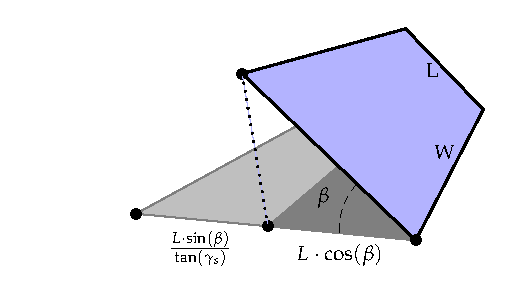
\includegraphics{../figs/DimensionesSeguidorSombra}
\end{centering}

\caption{\label{fig:DimensionesSeguidorSombra}Dimensiones de un seguidor a
doble eje y longitud de su sombra arrojada.}

\end{figure}


%
\begin{figure}
\begin{centering}
\includegraphics{../figs/SixTrackerShadow}
\end{centering}

\caption{\label{fig:SeisSeguidores}Posibles sombras en un conjunto de seis
seguidores.}

\end{figure}


Al calcular las sombras mutuas entre seguidores, un sistema puede ser
modelado como un grupo de seis seguidores distribuidos en una matriz
de dos filas en la dirección Norte-Sur (figura
\ref{fig:SeisSeguidores}).  Con este modelo pueden representarse todas
las posibles sombras que inciden en un seguidor perteneciente a este
sistema (suponiendo que no hay desnivel en el terreno y que todos los
seguidores están ubicados en la cuadrícula).  En esta planta "tipo"
pueden distinguirse tres situaciones de sombra: E-O o lateral, N-S o
delantera y diagonal o cruzada, en función del seguidor que produce el
bloqueo de radiación.  Para caracterizar cada situación de sombra se
empleará un factor $FS_{xx}$ calculado como la razón entre el área del
generador afectado por la sombra y el área total (así, $FS_{xx}$ es
cero en ausencia de sombra).  \nomenclature[FSeo]{$FS_{eo}$}{Factor de
  sombras en dirección Este-Oeste.}
\nomenclature[FSns]{$FS_{ns}$}{Factor de sombras en dirección
  Norte-Sur.}  \nomenclature[FSd]{$FS_{d}$}{Factor de sombras en
  dirección diagonal.}
%OJO
%Se supone que el factor de sombras resultante reduce exclusivamente 
%la componente directa de la radiación efectiva incidente en el generador afectado. 

Mediante consideraciones puramente geométricas es posible caracterizar 
los tres factores de sombra con las siguientes ecuaciones, en las que
emplearemos los valores normalizados de las distancias,
$l_{eo}=\frac{L_{eo}}{W}$ y $l_{ns}=\frac{L_{ns}}{W}$:

\begin{equation}
\begin{array}{c}
|l_{eo}\cdot\cos(\psi_{s})|<1\\
|l_{eo}\cdot\sin(\psi_{s})|<s\end
{array}
\Rightarrow
FS_{eo}=\frac{(1-|l_{eo}\cos(\psi_{s})|)\cdot(s-|l_{eo}\sin(\psi_{s})|)}{s}
\end{equation}


\begin{equation}
\begin{array}{c}
|l_{ns}\cdot\cos(\psi_{s})|<s\\
|l_{ns}\cdot\sin(\psi_{s})|<1
\end{array}
\Rightarrow 
FS_{ns}=\frac{(s-|l_{ns}\cos(\psi_{s})|)\cdot(1-|l_{ns}\sin(\psi_{s})|)}{s}
\end{equation}


\begin{align*}
\begin{array}{c}
s>|l_{ns}\cdot\cos(\psi_{s})|+|l_{eo}\sin(\psi_{s})|\\
1>|l_{eo}\cdot\cos(\psi_{s})|-|l_{ns}\cdot\sin(\psi_{s})|
\end{array} 
& \Rightarrow
\end{align*}
\begin{equation}
FS_{d}=\frac{\left[s-\left(|l_{eo}\cdot\sin(\psi_{s})|+|l_{ns}\cos(\psi_{s})|\right)\right]\cdot\left[1-\left(|l_{eo}\cdot\cos(\psi_{s})|-|l_{ns}\sin(\psi_{s})|\right)\right]}{s}
\end{equation}


siendo $\psi_{s}$ el acimut solar y $\gamma_{s}$ la altura solar y
donde la longitud de sombra (normalizada con la anchura del seguidor) se calcula con:

\begin{align}
s & =s_{1}+s_{2}\\
s_{1} & =b\cdot\cos(\beta)\\
s_{2} & =\frac{b\cdot\sin(\beta)}{\vert\tan(\gamma_{s})\vert}
\end{align}

El factor $\frac{\sin(\gamma_{s})}{\sin(\gamma_{s}+\beta)}$ representa 
la proyección de sombra existente en el suelo sobre el plano 
del generador, y por tanto, el porcentaje de área sombreada que 
debe ser eliminado de la radiación directa. Desarrollando este factor 
se obtiene una formulación alternativa que puede facilitar el cálculo de los tres factores:
\begin{align}
FS_{eo} & =\frac{(1-l_{eo}\cos(\psi_{s}))\cdot(s-l_{eo}\sin(\psi_{s}))}{s}\\
FS_{ns} & =\frac{(s-l_{ns}\cos(\psi_{s}))\cdot(1-l_{ns}\sin(\psi_{s}))}{s}\\
FS_{d} & =\frac{\left[s-\left(l_{eo}\cdot\sin(\psi_{s})+l_{ns}\cos(\psi_{s})\right)\right]\cdot\left[1-\left(l_{eo}\cdot\cos(\psi_{s})-l_{ns}\sin(\psi_{s})\right)\right]}{s}
\end{align}

Para un planta de seguimiento a doble eje se calcula la irradiación 
recibida por un seguidor \emph{promedio} como la media aritmética ponderada 
de la radiación recibida por los seis seguidores, según la proporción 
de seguidores que ocupan cada posición 
(por ejemplo, es evidente que una planta multimegawatio contará con
una alta proporción de seguidores en la posición del nº 5) 
(figura \ref{fig:SeisSeguidores}), siendo esta radiación \emph{promedio}
la base para el cálculo de la producción final de la planta. 
Nuevamente en la figura \ref{fig:SeisSeguidores} comprobamos que 
el seguidor 1 recibe sombra E-O del 2 por la tarde, 
mientras que el 3 la recibe del 2 por la mañana; 
el 2 recibe sombra E-O del 1 por la mañana y 
del 3 por la tarde (en la segunda hilera, la situación es idéntica). 
En lo que a sombras cruzadas se refiere, 
el seguidor 6 es sombreado por el 2 por la tarde, 
el 5 por el 1 por la mañana y por el 3 por la tarde, 
y por último, el seguidor 4 recibe sombra del 2 por la mañana. 
Un análisis equivalente integra el factor N-S en el calculo global.

Realizando la simulación de este sistema incluyendo el cálculo de
sombras, y repitiendo la simulación para varias combinaciones $(L_{ns,}L_{eo})$
pueden elaborarse gráficos de nivel%
\footnote{Implementados en la función
  \href{http://search.r-project.org/R/library/solaR/html/optimShd.html}{\texttt{optimShd}}
  de \texttt{solaR} \cite{Perpinan2012b}}%
 como el de la figura
\ref{fig:Abaco-para-planta}, donde se recoge el ratio entre
la energía anual producida por un seguidor \emph{promedio} incluyendo
el efecto de por sombras mutuas
\footnote{Recordemos
que en el cálculo de la producción del seguidor afectado por sombras
mutuas se considera que la reducción en potencia
está exclusivamente relacionada con el área sombreada, por tanto sin tener en
consideración las conexiones eléctricas entre módulos).}
y la energía anual producida por un seguidor sin sombreado. 

\begin{figure}
\begin{centering}
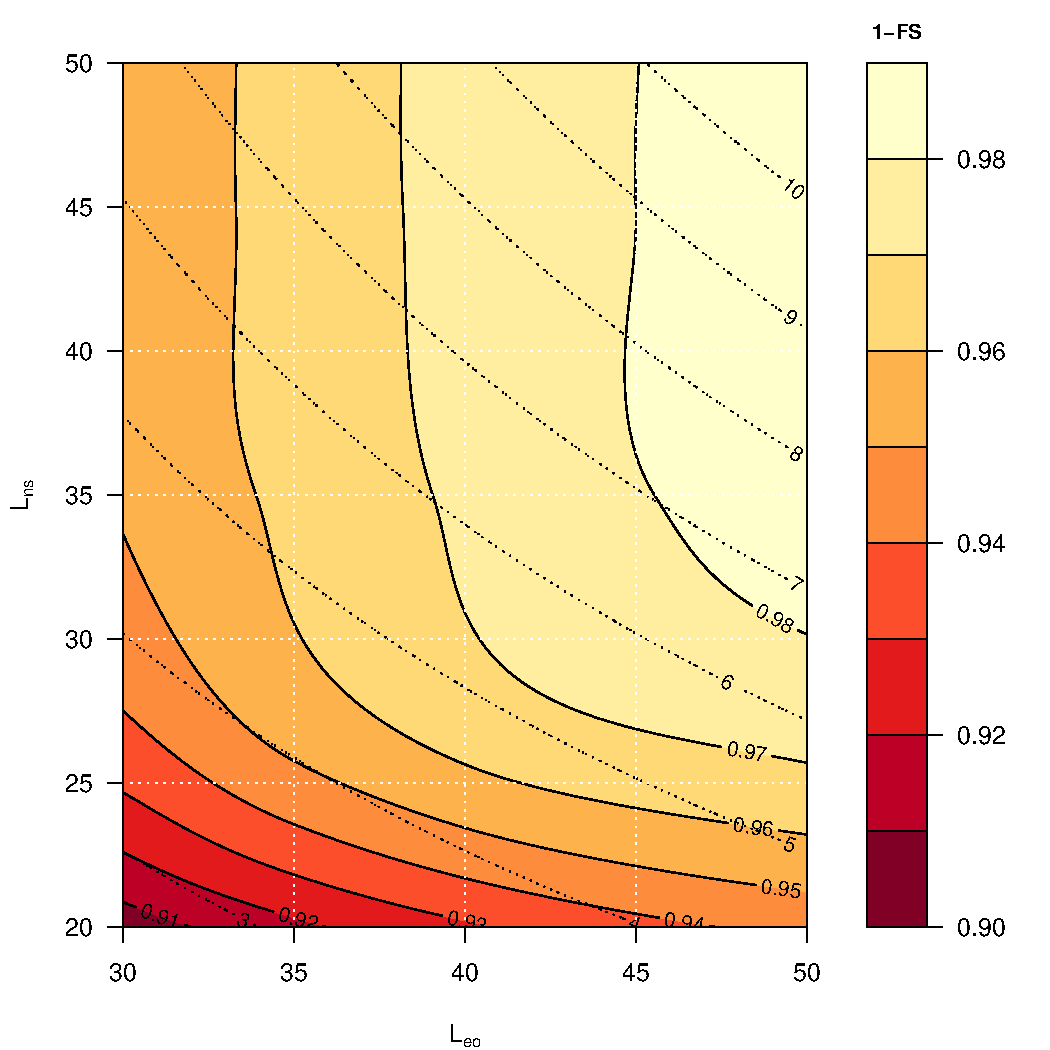
\includegraphics[scale=0.75]{../figs/AbacoSombras}
\end{centering}

\caption[Ábaco para planta de seguimiento a doble eje.]{Ábaco para
  planta de seguimiento a doble eje\label{fig:Abaco-para-planta}. 
Recoge el ratio entre la energía anual producida por un seguidor afectado por sombras mutuas
($E_{acS}$) y la producida por un seguidor sin sombreado ($E_{ac0}$). Las curvas
de color negro representan la fracción de energía no afectada por sombras.
Las curvas de puntos representan el valor del ROT. }
\nomenclature[Eac]{$E_{ac}$}{Energía entregada a la salida de un
  inversor}
\nomenclature[Eac0]{$E_{ac0}$}{Energía entregada a la salida de un
  inversor sin considerar las pérdidas por sombreado}
\nomenclature[EacS]{$E_{acS}$}{Energía entregada a la salida de un inversor considerando las pérdidas por sombreado}
\end{figure}


Una primera observación a la figura \ref{fig:Abaco-para-planta} permite
comprobar que existe un par ($L_{ns}$, $L_{eo}$) tal que, para una
determinada producción de energía, proporciona el mejor valor de ocupación
de terreno. Dicho de otra manera, una vez que se acepta un valor de
pérdida por sombras mutuas, a partir de cierto tamaño de cuadricula
carece de sentido aumentar la distancia entre seguidores. Esta figura
permite comprobar que valores de ROT comprendidos entre 5 y 6 son
razonables en cuanto a energía producida y a incremento de productividad
por aumento en la ocupación. De la línea correspondiente a $ROT=6$
(que, decíamos, era un valor característico de los sistemas a doble
eje) comprobamos que produce unas pérdidas cercanas al $2\%$. 

Como es de esperar, la aparición de sombras se produce al amanecer
y al atardecer (figura \ref{fig:CuadriculaFija}) siempre que la separación
entre seguidores no baje de un cierto umbral. Así, el seguidor \emph{promedio}
amanece recibiendo entre el $30\%$ y el $40\%$ de la radiación efectiva
que llega a un seguidor aislado, pero en un periodo de tiempo breve
queda libre de sombras hasta el atardecer. 

%
\begin{figure}
\begin{centering}
\includegraphics[scale=0.6]{../figs/SombrasDiaAno_Lns30Leo40}
\end{centering}

\caption[Evolución del sombreado en un seguidor
promedio]{\label{fig:CuadriculaFija}
Evolución del sombreado en un seguidor
promedio situado en una cuadricula. 
En la gráfica, el valor 0 indica
sombra total y el valor 1 ausencia de sombra.}

\end{figure}

\subsubsection{Sistemas de seguimiento de eje horizontal}

Consideremos que los seguidores son de longitud infinita en sentido
Norte-Sur (despreciamos el efecto de bordes). Así, los parámetros
que determinan el diseño de este tipo de sistema son (\ref{fig:SeguidorEjeHorizontalSombras}):

\begin{enumerate}
\item La inclinación del generador fotovoltaico, $\beta$, (coincidente
con el ángulo $\psi_{ns}$).
\item La dimensión en sentido Este-Oeste del campo generador, $L$.
\item La separación entre los diferentes seguidores en la dirección Este-Oeste,
$L_{eo}$. 
\end{enumerate}

Por tanto, $ROT=\frac{L_{eo}}{L}$.

\begin{figure}
  \centering
  \includegraphics[scale=0.9]{../figs/SombrasHoriz}
  \caption{Dimensiones básicas en sistemas con seguidores de eje horizontal.}
  \label{fig:SeguidorEjeHorizontalSombras}
\end{figure}

Para caracterizar numéricamente el sombreado, se empleará el factor
$FS_{eo}$. Mediante consideraciones geométricas, utilizando la
distancia normalizada $l_{eo}=\frac{L_{eo}}{L}$, es posible escribir:

\begin{align}
FS_{eo} & =\frac{s-l_{eo}}{s}\nonumber \\
 & =1-l_{eo}\cdot\cos(\beta)\nonumber \\
 &
 =1-l_{eo}\cdot\frac{\sin(\omega)}{\sqrt{\sin^{2}(\omega)+\left(\cos(\omega)\cos(\phi)+\tan(\delta)\sin(\phi)\right)^{2}}}\label{eq:FSeoHorizontal}
\end{align}

En este caso, la  configuración
de la planta consiste en elegir la distancia entre ejes de seguidores
contiguos. La figura \ref{fig:SeguidoresEjeHorizontalSeparacion}
muestra las pérdidas energéticas por sombreado mutuo para diferentes
separaciones entre ejes. Dado que la distancia está normalizada, esta gráfica relaciona las pérdidas con el ROT.
Nuevamente aparece una región de valores que representan un buen compromiso
entre energía producida y ocupación de terreno (alrededor de ROT=4
con pérdidas por sombreado inferiores al $4\%$). Superar este valor
de ocupación proporciona incrementos de producción muy bajos que desaconsejan
aumentar la separación. Por tanto, si para instalaciones de doble eje proponíamos el valor
de ROT=6, el valor elegido para instalaciones de eje horizontal N-S
es ROT=4.

\begin{figure}
  \centering
  \includegraphics[scale=0.7, angle=90]{../figs/AbacoSeguidorHorizSombra_Ene10}

  \caption{Separación entre seguidores de eje horizontal.}
  \label{fig:SeguidoresEjeHorizontalSeparacion}
\end{figure}

\subsubsection{Limitación de ángulo y retroseguimiento}
\label{sec:backtracking}

Como ha sido estudiado anteriormente, el sombreado en un generador puede producir problemas por
el efecto de \emph{punto caliente}. En seguidores de eje horizontal se puede evitar la incidencia
de sombras en cualquier instante mediante algoritmos de
\emph{backtracking} o retroseguimiento
\cite{Panico.Garvison.ea1991}. Esta técnica provoca el desvío del seguidor de su posición óptima en los
instantes en los que se produce la sombra entre seguidores, evitando
el impacto de sombras pero con la consiguiente reducción en energía
producida por alejamiento del apuntamiento óptimo.

Para evitar la
aparición de sombras, el ángulo de inclinación de los seguidores debe
ser tal que la longitud de la sombra sea igual a la distancia entre
seguidores. Denominemos con $\beta$ al angulo de inclinación con
retroseguimiento, y con $\beta_0$ al ángulo de inclinación
original. De la ecuación (\ref{eq:FSeoHorizontal}) se deduce que
sólo será necesario aplicar esta técnica cuando $l_{eo} \cdot \cos(\beta_0) \leq 1$. El
triángulo definido por el rayo solar, el seguidor y la sombra debe
cumplir la siguiente condición, basada en el teorema de los senos:

\begin{equation}
  \label{eq:BT_senos}
  \frac{l_{eo}}{\cos(\beta_0-\beta)}=\frac{1}{\cos{\beta_0}}
\end{equation}

Por tanto, el ángulo de inclinación que garantiza la ausencia de
sombras a costa de apartarse de la condición de seguimiento es:
\begin{equation}
  \label{eq:retroseguimiento}
  \beta=\beta_0-\arccos(l_{eo}\cdot\cos{\beta_0})  
\end{equation}
ecuación que debe aplicarse sólo cuando $l_{eo} \cdot
\cos(\beta_0) \leq 1$. En caso contrario $\beta = \beta_0$.

En la figura \ref{fig:Backtracking} se representa la evolución del
ángulo de inclinación de un seguidor de eje horizontal sometido a
retroseguimiento y, además, con limitación de su ángulo de
inclinación.  Al amanecer el seguidor está en posición
horizontal. Según avanza el día el seguidor gira en sentido
contrario al movimiento solar para evitar las sombras. En un
determinado momento se cruza con el sol y puede continuar el
movimiento convencional. En un instante de la tarde debe volver a
cambiar el sentido hasta la horizontal en la noche.  

\begin{figure}
  \centering
  \includegraphics[scale=0.7]{../figs/BackTracking}
  \caption{Retroseguimiento y limitación del ángulo de inclinación
    en seguidores de eje horizontal.}
  \label{fig:Backtracking}
\end{figure}


Por otra parte, por motivos estructurales es habitual limitar 
el ángulo de inclinación en seguidores 
de doble eje a valores máximos alrededor de $\SI{70}{\degree}$, principalmente como
técnica de protección frente al viento. Esta peculiaridad de funcionamiento
tiene semejanzas con la técnica de retroseguimiento por el hecho de
implicar un desvio de los seguidores de su posición óptima obteniendo
sombras más cortas que en el caso teórico.  El límite de inclinación 
de un seguidor industrial implica una red más densa
que en el caso teórico, siendo la cruz de la moneda la reducción en
la energía generada por incidencia no perpendicular. 
Siguiendo este razonamiento para seguidores de doble eje, cabe la posibilidad de
utilizar retroseguimiento en el movimiento cenital, y no sólo en
sentido acimutal, como es común en equipos de control comercial.

\subsubsection{Elección de separaciones}
\label{sec:EleccionSeparaciones}

Con mayor separación disminuyen las pérdidas por sombreado
mutuo y por tanto, aumenta la productividad del sistema. Sin embargo, aumentan los costes relacionados con
el área ocupada y los costes relacionados con los elementos de unión
entre estructuras (cableado, canalizaciones, zanjas). 
Por tanto, la separación óptima entre elementos (seguidores o estructuras
estáticas) es aquella que conduce al mínimo valor del coste
de la energía producida por el sistema. 

La determinación de la separación óptima es un ejercicio
particular que depende no sólo de la técnica de
seguimiento elegida, sino también de las condiciones económicas de los
elementos que componen el sistema. No debe olvidarse que, la
consideración de las condiciones del terreno (fronteras, irregularidades, vaguadas,
etc.) obliga, en general, a decantarse por una separación algo difrente al
resultado del ejercicio de optimización.  El lector interesado queda
invitado a la lectura de la referencia \cite{Perpinan2012}.


\subsubsection{Elección entre Sistemas}
\label{sec:eleccion-sistemas}

La elección entre sistemas estáticos y sistemas de seguimiento debe
tener en cuenta, además de la mejor productividad, otros
condicionantes como el coste del sistema, el mantenimiento asociado o
las necesidades de ocupación de espacio. 

El mejor aprovechamiento de terreno depende directamente del
porcentaje de radiación que quedará sombreada por los seguidores
cercanos. En general, cuanto más exacto es el método de seguimiento,
menos eficiente es su aprovechamiento de terreno: para un mismo valor
de radiación sombreada, la separación entre seguidores aumenta en
sistemas que apuntan mejor. De esta forma el espacio necesario es
superior para el seguimiento a doble eje que para el seguimiento en eje
horizontal Norte-Sur, y a su vez, mayor que para un SFCR estático. De
ahí que en determinados casos en los que existan limitaciones de
espacio disponible, pueda resultar interesante una técnica que ofrezca
menor productividad.


\section{Cálculo de la productividad de un SFCR}


La potencia entregada a la salida de un SFCR está determinada por los siguientes factores:

\begin{itemize}
\item La irradiancia efectiva incidente en el plano del generador,
  cuyo procedimiento de cálculo es el objeto de estudio del capítulo \ref{cha:Radiacion}.


\item La temperatura ambiente a la que está sometido el generador
  fotovoltaico. En ausencia de información detallada, puede asumirse
  un valor constante $T_a=\SI{25}{\celsius}$ en el caso de
  simulaciones anuales \cite{Perpinan.Lorenzo.ea2007}.  Si se dispone
  de los valores máximos y mínimos diarios, es posible sintetizar una
  secuencia intradiaria mediante una combinación de funciones coseno
  \cite{Huld.Suri.ea2006}\footnote{Implementado en la función
    \href{http://search.r-project.org/R/library/solaR/html/fTemp.html}{\texttt{fTemp}}
    de \texttt{solaR} \cite{Perpinan2012b}}.
  \nomenclature[Ta]{$T_{a}$}{Temperatura ambiente}
\item El impacto de sombras sobre el generador, tal y como ha sido
  explicado en la sección \ref{sec:sombras}.
\item El comportamiento eléctrico del generador fotovoltaico, según lo
  estudiado en los capítulos \ref{cha:Celula} y \ref{cha:AsociacionDispositivos}.
\item La curva de eficiencia del inversor y su ventana de búsqueda del
  MPP (sección \ref{InversorSFCR}).
\item La eficiencia del resto de componentes del sistema,
  principalmente cableado y transformador de BT/MT. Es práctica común
  considerar constantes las pérdidas asociadas al cableado (por
  ejemplo, $1.5\%$) y modelar el funcionamiento del transformador si
  se dispone de información al respecto, o asumir un valor constante
  de pérdidas (por ejemplo, $2.5\%$).
\end{itemize}

% \subsection{Estimación de la irradiancia efectiva}
%   \label{sec:Gef_SFCR}

%   La irradiancia efectiva incidente en el plano del generador se
%   calcula a partir de valores de irradiación global en el plano
%   horizontal definidos para el lugar en estudio. Estos valores están
%   recogidos en bases de datos de diferentes características (radiación
%   estimada a partir de imágenes de satélite, estaciones meteorológicas
%   terrenas, etc.)  con periodos de almacenamiento más o menos largo.

%   Para la elección de la base de datos debe resolverse el compromiso
%   entre cercanía de la medida al lugar de la instalación y larga
%   duración de la base temporal.  Debe tenerse en cuenta que las
%   discrepancias entre bases de datos pueden llegar a ser de hasta el
%   30\%, y por tanto, todos los resultados posteriores deben manejarse
%   sin perder la perspectiva de esta incertidumbre.  Por tanto, es
%   sumamente importante referenciar cualquier estimación de
%   productividad a la base de datos empleada para el cálculo.

%   El apellido de ``efectiva incidente'' indica que es el resultado de
%   tener en cuenta la inclinación y orientación del generador, y
%   también sus características físicas en cuanto a aprovechamiento de
%   la luz incidente. Por tanto, incluye las pérdidas por suciedad,
%   transmitancia del vidrio y reflexión por incidencia no
%   perpendicular. El procedimiento de cálculo de la irradiancia
%   efectiva a partir de la irradiación global en el plano horizontal se
%   sintetizan en la Tabla \ref{Tabla calculation
%     procedure}\footnote{Implementado en la función \href{http://search.r-project.org/R/library/solaR/html/calcGef.html}{\texttt{calcGef}} de
%     \texttt{solaR} \cite{Perpinan2012b}}.

% %
%   \begin{table}[p]
%     \caption{Procedimiento de cálculo de la irradiancia efectiva.}
%     \label{Tabla calculation procedure}
%   \begin{tabular}{>{\raggedright}m{6cm}>{\raggedright}m{9cm}}
%     \toprule 
%     Paso & Método\tabularnewline
%     \midrule 
%     {\footnotesize Descomposición de radiación horizontal global en componentes
%       directa y difusa.} & {\footnotesize Correlación entre la fracción de difusa y el índice
%       de claridad. Para valores diarios es de uso común la propuesta de
%       Collares-Pereira y Rabl \cite{Collares-Pereira.Rabl1979} mientras
%       que para medias mensuales de valores diarios se emplea frecuentemente
%       la propuesta de Page \cite{Page1961}.}\tabularnewline
%     \midrule 
%     {\footnotesize Estimación de irradiancia a partir de valores diarios
%       de irradiación.} & {\footnotesize Generador empírico de perfil diario de irradiancia
%       a partir de valores de irradiación global \cite{Collares-Pereira.Rabl1979}.}\tabularnewline
%     \midrule 
%     {\footnotesize Transposición de irradiancia en el plano horizontal
%       a la superficie inclinada.} & {\footnotesize El cálculo de la radiación directa emplea exclusivamente
%       consideraciones geométricas. El tratamiento de la radiación difusa
%       necesita modelar el comportamiento de la esfera celeste. Un modelo
%       anisotrópico recomendable es el de Hay y McKay \cite{Hay.McKay1985}.}\tabularnewline
%     \midrule 
%     {\footnotesize Irradiancia del albedo.} & {\footnotesize Puede modelarse como una irradiancia difusa isotrópica
%       con un factor de reflexión igual a 0.2 (modificable si se dispone
%       de información del terreno).}\tabularnewline
%     \midrule 
%     {\footnotesize Efectos de la suciedad y el ángulo de incidencia.} & {\footnotesize Son recomendables las ecuaciones propuestas por Martín
%       y Ruiz \cite{Martin.Ruiz2001}.}\tabularnewline
%     \midrule
%     {\footnotesize Efecto del sombreado.} & {\footnotesize Es razonable suponer que el sombreado sólo afecta a
%       la componente directa de la irradiancia. Por otra parte, una posible
%       aproximación consiste en considerar que las pérdidas por sombra no
%       afectan al comportamiento eléctrico del generador y es suficiente
%       considerarlas en el cálculo de radiación: \[
%       G_{efs}=D_{ef}+R_{ef}+B_{ef}\cdot(1-FS_{xx})\]}\tabularnewline
%     \bottomrule
%   \end{tabular}
% \end{table}
% \nomenclature[Gefs]{$G_{efs}$}{Irradiación (o irradiancia)
%         global efectiva incidente en un generador considerando las
%         sombras}
% \nomenclature[Def]{$D_{ef}$}{Irradiancia difusa
%         efectiva incidente en un
%         generador}
% \nomenclature[Bef]{$B_{ef}$}{Irradiancia directa
%         efectiva incidente en un generador}

% Para el caso particular de los sistemas de conexión a red
% \emph{estáticos}, el procedimiento de la tabla \ref{Tabla calculation
%   procedure} puede ser aproximado mediante dos regresiones que
% relacionan la irradiación anual global efectiva con la irradiación
% anual global en el plano horizontal \cite{Caamano1998,Lorenzo2002,
%   Lorenzo2006c}. En primer lugar, se estima la relación entre la
% irradiación en el plano horizontal con la incidente en un generador
% con orientación e inclinación óptimas:

% \begin{equation}
%   \frac{G_{a}(0)}{G_{a}(\beta_{opt})}=1-4.46\cdot10^{-4}\cdot\beta_{opt}-1.19\cdot10^{-4}\cdot\beta_{opt}^{2}
%   \label{eq:GbetaOpt}
% \end{equation}

% A continuación, se obtiene la irradiación efectiva a partir de la
% incidente para el ángulo óptimo de inclinación:

% \begin{align}
%   \frac{G_{efa}(\beta,\alpha)}{G_{a}(\beta_{opt})} & =g_{1}\cdot(\beta-\beta_{opt})^{2}+g_{2}\cdot(\beta-\beta_{opt})+g_{3}\label{eq:Gef_estefania}\\
%   g_{i} &
%   =g_{i1}|\alpha|^{2}+g_{i2}|\alpha|+g_{i3}\label{eq:Gef_estefania_coef}
% \end{align}

% En estas ecuaciones los ángulos $\beta_{opt}$, $\beta$ y $\alpha$
% están en grados.

% Los coeficientes para resolver las ecuaciones \ref{eq:Gef_estefania} y
% \ref{eq:Gef_estefania_coef} son los recogidos en la tabla
% \ref{tab:CoefGef} para el caso de un módulo con suciedad media.

% \begin{center}
% %
%   \begin{table}
%     \begin{centering}
%       \begin{tabular}{cccc}
%         \toprule 
%         & $i=1$ & $i=2$ & $i=3$\tabularnewline
%         \midrule
%         \midrule 
%         $g_{1i}$ & $8\cdot10^{-9}$ & $3.8\cdot10^{-7}$ & $-1.218\cdot10^{-4}$\tabularnewline
%         \midrule 
%         $g_{2i}$ & $-4.27\cdot10^{-7}$ & $8.2\cdot10^{-6}$ & $2.892\cdot10^{-4}$\tabularnewline
%         \midrule 
%         $g_{3i}$ & $-2.5\cdot10^{-5}$ & $-1.034\cdot10^{-4}$ & $0.9314$\tabularnewline
%         \bottomrule
%       \end{tabular}
%       \par\end{centering}

%     \caption{Valores de los coeficientes de la ecuación \ref{eq:Gef_estefania_coef}
%       necesarios para resolver la ecuación \ref{eq:Gef_estefania} para
%       el caso de un módulo con suciedad media.\label{tab:CoefGef}}

%   \end{table}

%   \par\end{center}

\subsection{Energía Producida por un Sistema Fotovoltaico conectado a
  la Red}

A partir de la secuencia de valores de irradiancia efectiva y
temperatura ambiente, se calcula el funcionamiento del generador
(tensión y corriente MPP, y por tanto potencia), del inversor, del
cableado y del transformador (si lo hubiese). Estas secuencias
intradiarias de \emph{potencia} pueden ser integradas en períodos de
tiempo adecuados para obtener las correspondientes estimaciones de
\emph{energía} producida en base diaria, mensual o anual.

El cálculo detallado según este procedimiento exige la ayuda de
herramientas software que implementen cada paso\footnote{Implementado en la
  función \href{http://search.r-project.org/R/library/solaR/html/prodGCPV.html}{\texttt{prodGCPV}} de \texttt{solaR} \cite{Perpinan2012b}}. Sin embargo, la
energía producida por un SFCR en un período anual puede ser estimada,
de forma aproximada, con la ecuación \ref{eq:EnergiaSFCR}:

\begin{equation}
  E_{ac}=P_{g}^{*}\cdot\frac{G_{ef,a}}{G_{stc}} \cdot PR \cdot (1-FS)
  \label{eq:EnergiaSFCR}
\end{equation}
\nomenclature[Gefa]{$G_{ef,a}$}{Irradiación global
  efectiva anual incidente en un generador}
\nomenclature[PR]{$PR$}{Rendimiento global de un sistema de conexión a
  red (performance ratio)}
donde $E_{ac}$ es la energía producida anual ($\si{\kWh}$), $G_{stc}$
es la irradiancia en condiciones estándar de medida (STC,
$G_{stc}=\SI{1}{\kW\per\meter\squared}$,
$T_c=\SI{25}{\celsius}$), $P_{g}^{*}$ es la potencia nominal del
generador FV ($\si{\kilo\Wp}$) en condiciones estándar de
medida, $G_{ef,a}$ es la irradiación efectiva anual incidente en el
plano del generador ($\si{\kWh\per\meter\squared}$), $PR$ es el
rendimiento del sistema o \emph{performance ratio }y $FS$ es el factor
de sombras, siendo estos dos últimos parámetros adimensionales.

Frecuentemente se utiliza la productividad del sistema, $Y_{f}$, que
es el cociente entre energía producida y la potencia nominal del
generador fotovoltaico: 

\begin{equation}
  Y_{f}=\frac{E_{ac}}{P_{g}^{*}}\,\si[per-mode=fraction]{\kWh\per\kWp}
\end{equation}

\nomenclature[Yf]{$Y_{f}$}{Productividad de un sistema fotovoltaico}

Es importante resaltar que el valor de la potencia nominal que se
emplea en las ecuaciones anteriores, $P_g^*$, resulta de multiplicar
la potencia nominal de un módulo, según lo recogido en su ficha
técnica, por el número de módulos que componen el generador. De esta
forma, este valor de potencia nominal supone que todos los módulos que
componen el generador son idénticos y que su potencia es la que se especifica en la ficha de
técnica. Las pérdidas por dispersión de parámetros y las
debidas a la tolerancia de potencia quedan incluidos dentro del
\emph{performance ratio} (tabla \ref{tab:PR}).


\subsection{Pérdidas en el Sistema}

El \emph{performance ratio} (PR) es un factor concebido para incluir
todas las pérdidas de un sistema fotovoltaico que no tienen
dependencia con las condiciones meteorológicas. De esta forma, este
factor puede caracterizar el funcionamiento de un sistema durante un período
independientemente de la localidad en la que se ubica. En sentido
estricto esta afirmación no se corresponde con la realidad porque
algunas pérdidas incluidas en el PR tienen relación con la
climatología del lugar. En particular, es destacable el efecto de la
temperatura en la potencia entregada, y de ahí que este factor de
mérito varíe de un día al siguiente o de un mes a otro. 

Sin embargo, el uso del PR se realiza normalmente para caracterizar
períodos anuales. En este contexto, y dado que la influencia de la
temperatura es un factor de segundo orden comparado con la relación entre
energía e irradiación, suele aceptarse que el PR anual sirve para
caracterizar la calidad de un sistema fotovoltaico.  

Las pérdidas que habitualmente incluye un PR anual son las que se
recogen en la Tabla \ref{tab:PR}. El análisis de funcionamiento de diversos sistemas FV europeos llevado
a cabo por la Agencia Internacional de la Energía
\cite{Clavadetscher.Nordmann2007} ha mostrado que el rango de valores
que toma el \emph{performance ratio} anual es bastante amplio, con mínimos
de 0,4 y máximos de 0,85. Para sistemas instalados desde 1996, el
valor promedio de esta base de datos europea ha sido de 0,74.
%
\begin{table}
  \caption{Factores de pérdidas incluidos en el \emph{performance
      ratio} anual junto
    con valores recomendados.\label{tab:PR}}

\begin{tabular}{>{\centering}p{8cm}c}
  \toprule 
  Factor de pérdidas & Valor\tabularnewline
  \midrule
  \midrule 
  Dispersión de parámetros entre los módulos que componen el generador  & 2-4\%\tabularnewline
  \midrule 
  Tolerancia de potencia de los módulos respecto a sus características
  nominales  & 3\%\tabularnewline
  \midrule 
  Temperatura de funcionamiento de los módulos  & 5-8\%\tabularnewline
  \midrule 
  Conversión DC/AC realizada por el inversor & 8-12\%\tabularnewline
  \midrule 
  Efecto Joule en los cables  & 2-3\%\tabularnewline
  \midrule 
  Conversión BT/MT realizada por el transformador & 2-3\%\tabularnewline
  \midrule 
  Disponibilidad del sistema  & 0,5-1\%\tabularnewline
  \bottomrule
\end{tabular}
\end{table}





%%% Local Variables:
%%% mode: LaTex
%%% TeX-master: "ESF.tex"
%%% End: 
